\documentclass[12pt,oneside]{jsbook}
\bibliographystyle{junsrt}
\usepackage{amsmath,amsthm,amssymb}
\usepackage{arydshln}
\usepackage{multicol}
\usepackage[dvipdfmx]{graphicx}
\usepackage{comment}
\usepackage{bm}
\usepackage{caption}
\newcommand{\argmax}{\mathop{\rm arg~max}\limits}
\newcommand{\argmin}{\mathop{\rm arg~min}\limits}
\usepackage{epsfig}
%\setlength{\textheight}{186mm}
\setlength{\columnseprule}{0.3pt}
\begin{document}
\pagestyle{empty}
\begin{center}
\vspace*{3cm} \underline{\HUGE 卒業論文} \\
\vspace{0.5cm}
\bf{ \Huge アンテナ特性に起因した異方性を\\
\Huge 軽減する複素自己組織化マップを\\
\Huge 用いた1次元アレイアンテナ式\\
\Huge 地雷可視化システム }\\
\vspace{0.5cm}
\huge 平成27年2月6日提出 \\
\vspace{3cm}
\huge 指導教官 \hspace{5cm} 廣瀬 明 教授 \\
\vspace{2cm}
\huge 電気電子工学科 \\
\vspace{1cm}
\huge 120472 \hspace{5cm} 小山 英利香
\end{center}


\newpage 
\setcounter{page}{1}
\pagestyle{headings}
\tableofcontents

\newpage 
\chapter{序章}
\section{研究背景}
\subsection{地中探査レーダによる地雷探査}
電磁波を用いた地中探査レーダ(Ground-Penetrating Radar:GPR)は探査対象へ
の非接触・非破壊探知が可能なため,埋設物探査や地下水調査など多くの分野で
用いられている\cite{Arai}\cite{2007TCounts}.同様に,プラスチックなどの非金属で製作された地雷の探査に
も活用できる技術として,広く研究の対象となっている\cite{chichi}\cite{JeroenYarovoy}\cite{YaroboyLighthart}\cite{2004MSato}
\cite{2005Sato}\cite{2009Sato}.

しかしGPRを用いた地雷探査には以下の難点がある.
\begin{enumerate}
\item 対象となる地雷が小型である
\item 金属に比べて反射率が低い
\item 地中の浅い部分を探査するために地表面の影響が相対的に大きい
\item ほかの散乱体が存在する
\end{enumerate}
これらの要因により,散乱波の位相と振幅のデータだけで
埋設された地雷を直接特定することは難しい.
\subsection{地雷可視化システム}
先述の問題に対して,本研究室ではGPRの散乱波により得られた地雷に特有のテクスチャ
の特徴量を複素自己組織化マップ(Complex-valued Self-Organizing Map : CSOM)
によって特定することで,地雷を可視化するシステムを実現させた
\cite{2007SMas}\cite{2008SMas}\cite{2009Nakano}\cite{2010Nakano}.

地雷可視化のプロセスは,以下に示す様に4段階に分けられる.
\begin{enumerate}
 \item マイクロ葉送受信のフロントエンドにより地表面からの散乱波データを取得する
 \item 取得されたデータに前処理をして複素テクスチャ特徴量ベクトルを計算,抽出する
 \item 抽出されたテクスチャ特徴量ベクトルをCSOMにかけて適応的に分類する
 \item 区分化された特徴量に対して地雷らしさを評価する
\end{enumerate}
ベクトルネットワークアナライザがマイクロ波を発生させ,スイッチの
切り替えにより1つのアンテナにマイクロ波が導かれ送信される.散乱波
は別の1つのアンテナが受信し,スイッチを通ってベクトルネットワークアナラ
イザで観測される.
取得したデータはノート型パーソナルコンピュータに転送され,そこで解析が行
われる.

しかし,本システムには
\begin{enumerate}
 \item メンテナンスに時間がかかる
 \item 反復使用で寿命が短い
 \item 計測に時間がかかる
 \item 直接結合の影響が大きい
\end{enumerate}
という課題が残されていた.

\section{目的}
本研究では上記課題を解決する
新しいシステムを用いて実際に地中を測定し,自己組織
化マップを適用して従来の2次元アレイアンテナ式地雷可視化システムと遜色な
く地雷を可視化することを目標とする.本稿では新型となる1次元アレイアンテ
ナ式地雷可視化システムに加えた改良を報告し,新しいフロントエンドに起因する問題
をソフトウェア面で解決する手法を提案する.
\newpage
\chapter{地雷可視化システム}
\section{従来のフロントエンド}
システムの概要を図~\ref{pic:const_ov}に示す.システムはアンテナ部,スイッ
チング部,画像処理部から構成されている.フロントエンドはタワー状になっており,底面にアンテナが取り付けられ
ていたため,フロントエンドを持ち上げて計測したい地表の真上に持っていく必要があっ
た.
\begin{figure}[hbtp]
\begin{center}
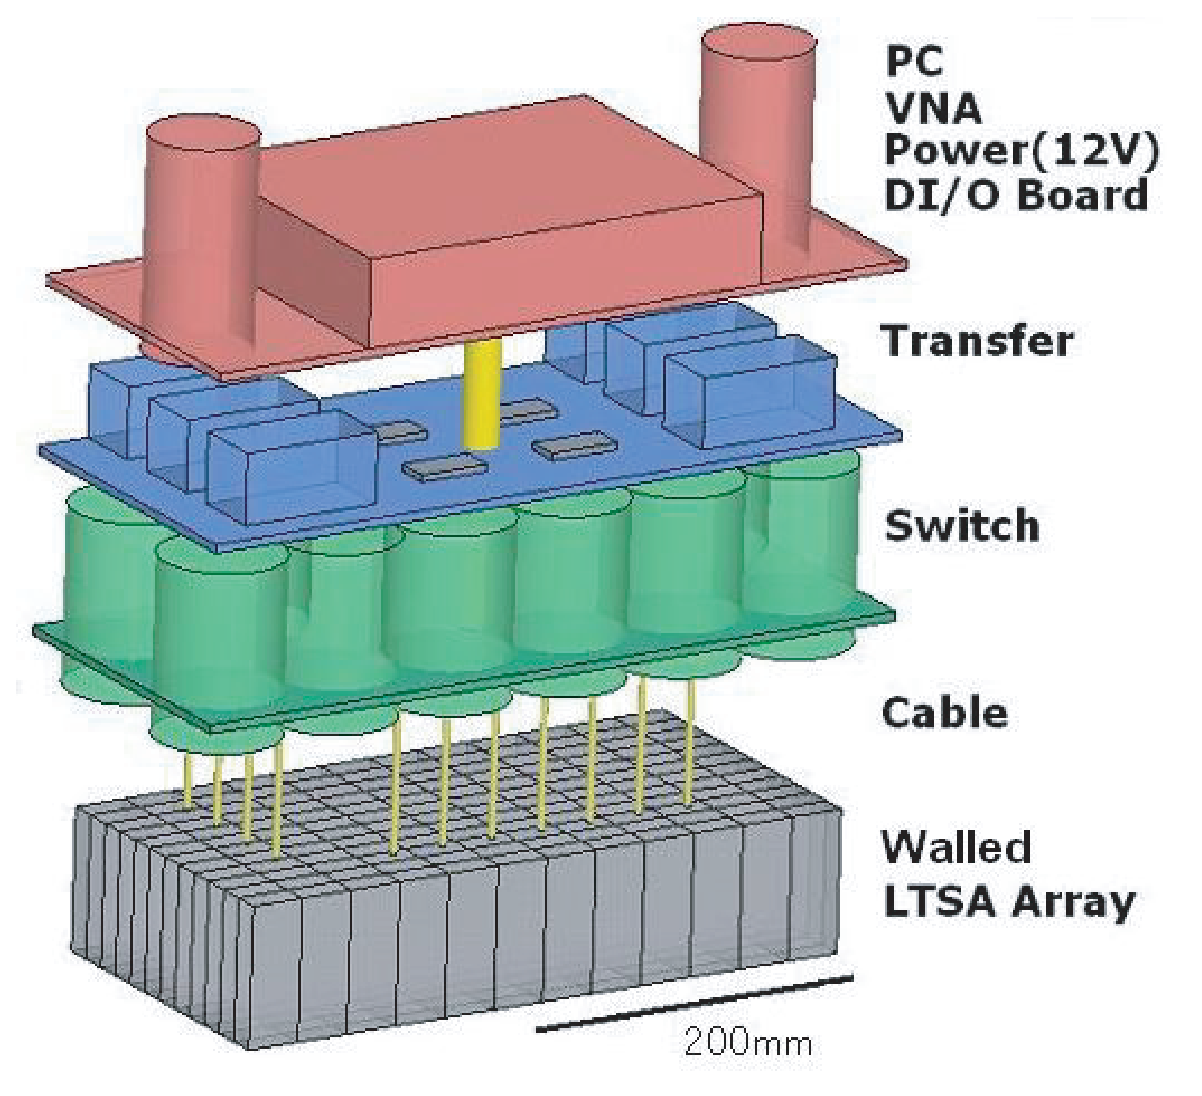
\includegraphics[width = 0.6\hsize]{so1.eps}
\caption{2次元アレイアンテナ式地雷可視化システムの概要図} \label{pic:const_ov} 
\end{center}
\end{figure}

アンテナ部は図~\ref{pic:transmit}のようになっており,Walled Linearly Tapered Slot Antenna (LTSA)\cite{2007SMas}が使われている.
このアンテナは広帯域かつ高ゲインであり,近接場イメージングに適
している.このシステムにおいてGPRに用いる周波数帯は8$\sim$12[GHz]で,8[G
Hz]から0.4[GHz]刻みで散乱波を取得する.
アンテナ部はこのアンテナを12個ずつ2次元に144個並べた
構造をしている.

\begin{figure}[hbtp]
\begin{center}
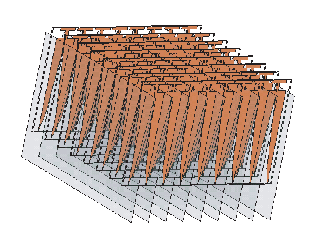
\includegraphics[width=0.6\hsize]{LTSA.eps}
\caption{アンテナ部の全体図} \label{pic:transmit} 
\end{center}
\end{figure}
ベクトルネットワークアナライザで発生させたマ
イクロ波をスイッチングで指定したアンテナから送信する.マイクロ波が地面や
地中の散乱体により散乱し,この散乱波を同じくスイッチングで指定したアンテ
ナで受信する.受信したデータはベクトルネットワークアナライザからコンピュー
タに送られる.散乱波はx,yの空間的2次元領域と周波数領域の3次元の
データになっており,これを画像として扱う.画像処理部では
測定データをSelf-Organizing Map(SOM)によって処理し,区分化する.
以降のソフトウェア面での処理は
\ref{021920_15Feb15}で説明する.

ここで,本システムの課題について述べる.
まず,メンテナンスに非常に時間がかかるというのは,配線が増えるとコネクタ
部の故障に対応する手間も増えるためである.また,本システムには信号の減衰
が少ない理想的なスイッチ
である高周波用のメカニカルスイッチ20個が多層化されて用いられ,これがさ
まざまな送受信の組み合わせを可能にしていた\cite{2008SMas}
が,機械式であるために電子スイッチに比べ反復使用で壊れやすいという難点
もあった.同時に,機械式スイッチは切り替えに時間がかかり,上記505点の計
測に22分を要していた.
さらに高密度にアンテナを配置しているため,直接結合の影響を物理
的に極力排除することを考えたWalled LTSAでも,実際には直接結合の影響が無
視できないほど大きく出ていた.
これらの問題を回避するために,新しいフロントエンドが提案された.


\subsection{以前提案した1次元アレイアンテナ式地雷可視化システム}\label{1array_before}
前節で提案されたと述べた1次元アレイアンテナ式地雷可視化シ
ステム\cite{ejiri}(図\ref{so2})は以下のコンポーネントによって構成される.
\begin{enumerate}
\item 1次元アレイ状のフロントエンド
\item 電子式スイッチ
\item 機械式スイッチ
\item ベクトルネットワークアナライザ
\end{enumerate}

フロントエンドにはTaper-Walled LTSA(図\ref{pic:twltsa}(b))が使われている.
このLTSAは我々の研究室で製作されたものであり,同じく以前我々の研究室から
提案したWalled LTSA(図\ref{pic:twltsa}(a))よりも更に直接結合が軽減されて
いる\cite{2011Nakano}.
\begin{figure}[btp]
 \begin{center}
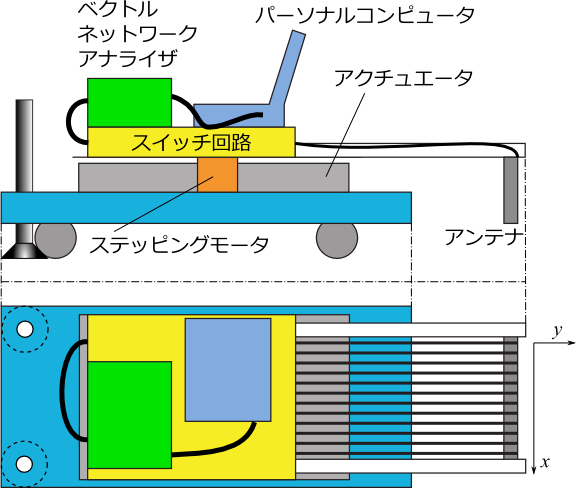
\includegraphics[width =0.6\hsize ]{so2.png}
\caption{1次元アレイアンテナ式地雷可視化システム}
\label{so2}
  \end{center}
\end{figure}
\begin{figure}[btp]
\begin{center}
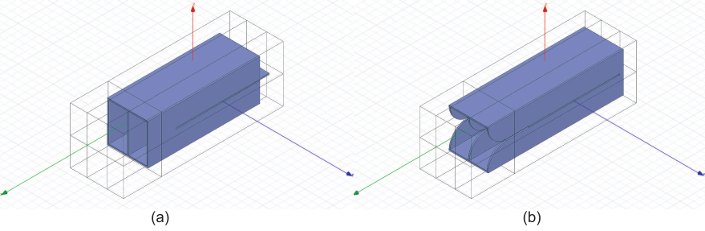
\includegraphics[width =\hsize]{walled-taper.png}
\caption{Walled LTSAとTaper-Walled LTSA} \label{pic:twltsa} 
\end{center}
\end{figure}
アンテナを1列に配置することにより,アンテナ数を144から12に,
メカニカルスイッチ数を20から5に減らした.配線数,高周波用コネク
タの数も大幅に削減することができ,信頼度が向上した.

このシステムのスイッチング回路には一部にpinダイオードスイッチが使用されて
いる(図\ref{scircuit}).pinダイオードとは一般のダイオードに用いられるP
層とN層の間に真性半
導体のI層がある3層構造となっているダイオードで,高周波におけるスイッチ
特性に優れているために広く使われている.しかしpinダイオードは信号の減衰
が大きいために,このシステムでは高速かつ頻繁な切り替えが求められる部分に
これを使用し,それほど切り替えが頻繁である必要がない部分にはメカニカルス
イッチを用いることで,信号の減衰を抑えつつ,計測時間を短縮し,長寿命化と
保守性の向上を目指した.

\begin{figure}[btp]
\begin{center}
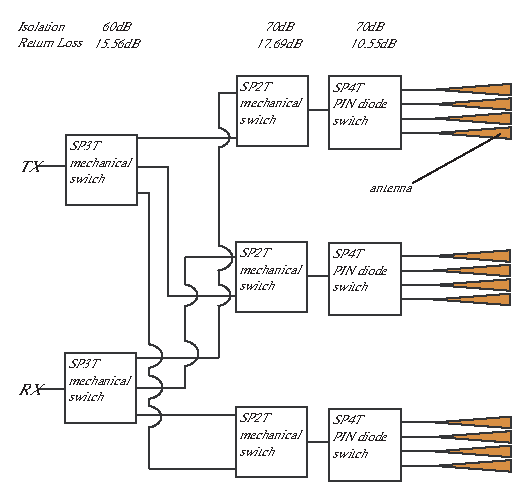
\includegraphics[width =0.8\hsize ]{switch-circuit.eps}
\caption{スイッチング部の回路図}
\label{scircuit}
 \end{center}
\end{figure}

また,データ点の取り方は図\ref{so2get}のようになっている.
アンテナを1次元に配列し($x$方向),アクチュエータにより直交方向
($y$方向)にアンテナを動かすことで,2次元に画像を取得できる.
従来のシステム
では送信アンテナに対し受信アンテナを1つ隣,2つ隣,1つ下,1つ斜め下とした
4種類505点のデータを取得したが,新型のシステムでは1つ隣,2つ隣の2種類のデー
タしか取れない.これは一見して情報量が減少しているようだが,サーボを用いてアン
テナを自由に前後に動かせるため,実際には同程度の情報量を得ることができる.
実験では,一列のアンテナで21点の計測が可能であることを受けてサーボ
の進行方向にもアンテナの列長14.3cmと近い14.7cmの間に22点のデータを取ることとし,
462点のデータを得た.
\begin{figure}[btp]
 \begin{center}
 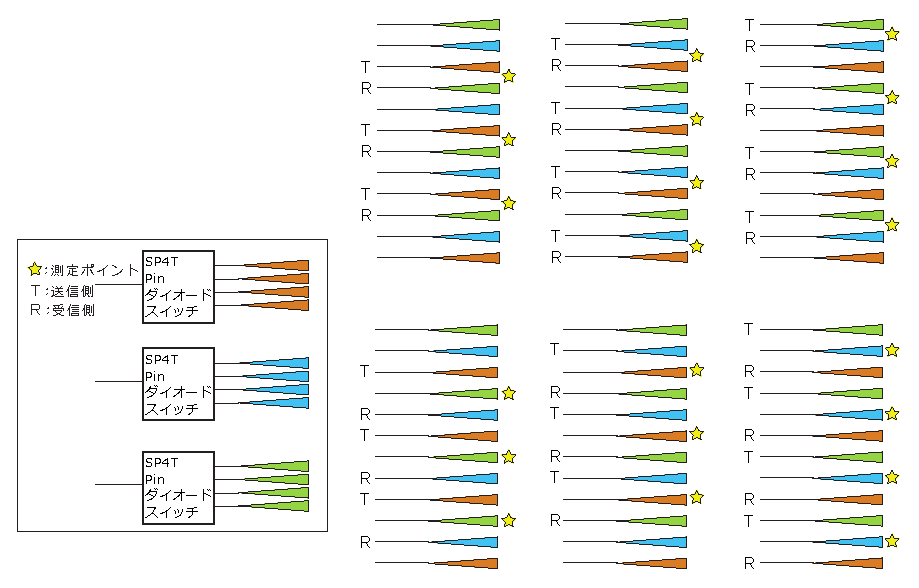
\includegraphics[width =\hsize ]{switch-circuit2.eps}
\caption{データ取得方法}
\label{so2get}
 \end{center}
\end{figure}
\newpage
\section{可視化処理}
\label{021920_15Feb15}
\subsection{前処理}
フロントエンドから得られるデータには,アンテナの個体差,使用するスイッチ
やケーブルの違いによる経路差,アンテナ間の直接結合の3つのノイズの影響がある.
これらを補正するために,事前に補正用のデータを取得し
ておく.これにはアンテナを電波吸収体を敷いた床から90cm上げて
周囲に何もない状態で計測したものを用いる.
得られるデータは複素数$z_{raw}$,補正用のデータは$z_{coup}$である.
これに対し直接結合を以下の式に従い補正し,補正後のデータ$z_{after}$を得る.

\begin{equation}
 z_{tmp}(x,y,f)=z_{raw}(x,y,f)-z_{coup}(x,y,f)
\end{equation}
\begin{equation}
 z_{after}(x,y,f)=\exp(-i\theta_{path})\cdot\exp(-i\angle z_{coup}(x,y,f))\cdot z_{tmp}(x,y,f)
\end{equation}
\begin{equation}
 \theta_{path}=\frac{2\cdot2\pi}{\lambda} \sqrt{d^2+h^2}
\end{equation}
ここで,$d$,$h$とは図\ref{dc}に示した部分の長さである.ただし$h$は
実際には分からないため,地表までの距離である4cmを採用した.
なお従来は,振幅の減衰差はそれほどないものとし,位相にのみ直接結合の補正
を行なっていた.
\begin{figure}[btp]
 \begin{center}
  \begin{tabular}{c}
   \begin{minipage}{0.4\hsize}
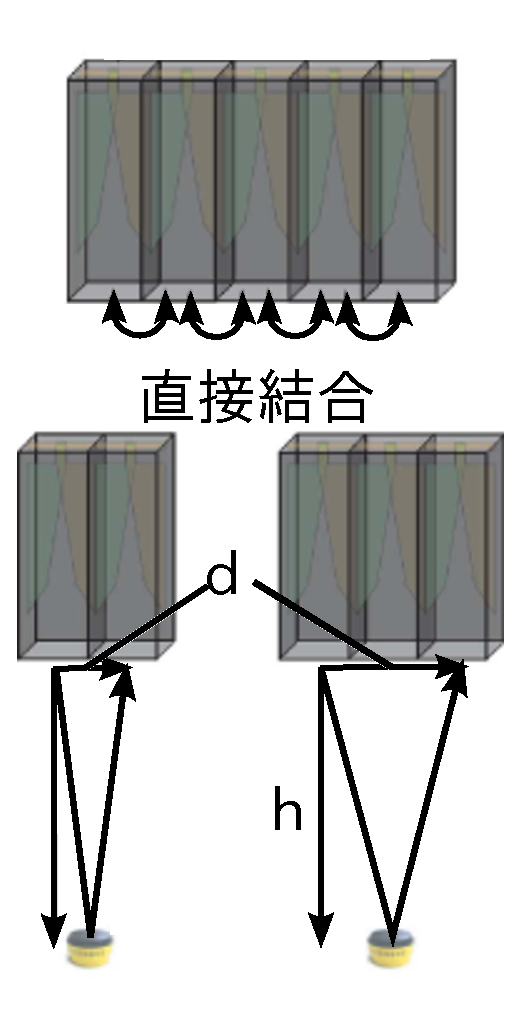
\includegraphics[width =\hsize ]{directcoup.eps}
\caption{直接結合と補正のための経路長}
\label{dc}      
   \end{minipage}
   \begin{minipage}{0.6\hsize}
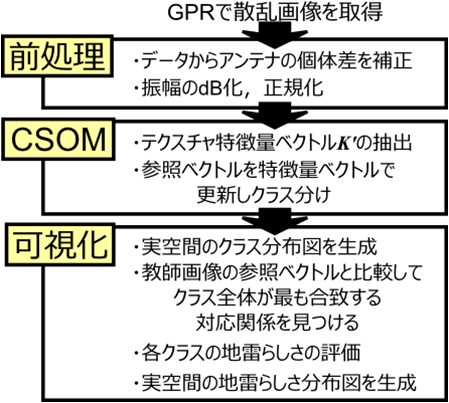
\includegraphics[width =\hsize ]{flowchart.png}
\caption{データ取得から地雷可視化までの流れ}
\label{flow}          
   \end{minipage}
  \end{tabular}
 \end{center}
\end{figure}

直接結合の補正の後,振幅をlogスケールにしてdBで表して人間の目の感覚に近づけ,
それを正規化
する.ここまでを前処理とし,これによって得られたデータをSOMに掛けて
区分化を行う.
\subsection{CSOMを用いた地雷可視化}
SOMとはニューラルネットワークの一種で,与えられた入力情報の類似度を
マップ上の距離で表現するモデルである.
SOMは複数のニューロンで構成される.各ニューロンは入力ベクトルと同次元の
参照ベクトルを持つ.
SOMに入力ベクトルとなる特徴量ベクトルが与えられると,特徴量ベクトルに
最も近い参照ベクトルを持
つニューロンが勝者となる.このとき,座標空間上でより勝者の近くに位置する
ニューロンほど強く学習し,その強さに応じて自身の参照ベクトルを特徴量ベクト
ルに近づける.このように参照ベクトルの更新を繰り返し,ベクトル空間上での
参照ベクトル同士の関係性が座標空間上で表現される.

本システムでは,ニューロンを1次元のリン
グ状に配置したRing-SOMを用いる.また,複素数のデータを扱うため,複素数に
対応したSOMであるCSOM(Complex-valued SOM)を利用している
.測定データから特徴量ベクトルを抽出し,SOMを利用して各ピ
クセルの類似度を1次元の値として表現する.

\subsection{特徴量ベクトルの抽出}
CSOMでは局所的テクスチャを見て分類する.
まず,$L\times L$ピクセルの局所ウィンドウを設定して,
テクスチャ特徴量を抽出する.
今回は$L=4$としている.
その後,$(x,y)$について掃引し,特徴量ベクトル${\bm K}(x,y)$を次のように得る.
\begin{eqnarray}
{\bm K} = \left[\begin{array}{ccc}
      {\it K_{{\rm m}}} & {\bm K_{{\rm s}}} & {\bm K}_{{\rm f}}
           \end{array} \right]^{\mathrm{T}}\label{eq.K}
\end{eqnarray}
ただし$T$は転置を表す.
位置$(x,y)$における${\bm K}(x,y)$は,空間的なテクスチャ特徴量
${\it K_{{\rm m}}},{\bm K_{{\rm s}}}$と周波数領域のテクスチャ特徴量
${\bm K_{{\rm f}}}$からなる.
空間的なテクスチャ特徴量は,
各$(l_x,l_y)$の複素画素値の平均${\it K_{{\rm m}}}$,$(l_x,l_y)$の自己相関
${\it K_{{\rm s}}}(0,0)$,$(l_x,l_y)$と$(l_x,l_y+1)$,$(l_x+1,l_y)$,
 $(l_x+1,l_y+1)$との相互相関${\it K_{{\rm s}}}(0,1),
 {\it K_{{\rm s}}}(1,0),{\it K_{{\rm s}}}(1,1)$をとる.
\begin{eqnarray}
 {\it K_{{\rm m}}} &=& \frac{1}{L^{2}N}\sum_{l_x = 1}^{L}\sum_{l_y =
 1}^{L}\sum_{n = 1}^{N}z\left(l_x, l_y, f_0 + nf_{{\rm int}}\right)\\
{\bm K_{{\rm s}}} &=& \left[\begin{array}{cccc}
 {\it K_{{\rm s}}}(0,0) & {\it K_{{\rm s}}}(0,1) &
 {\it K_{{\rm s}}}(1,0) & {\it K_{{\rm s}}}(1,1)
 \end{array} \right]^{\mathrm{T}}
\end{eqnarray}
\begin{eqnarray}
 {\it K_{{\rm s}}}(i,j) = \frac{1}{L^2N}\sum_{l_x = 1}^{L}\sum_{l_y =
 1}^{L}\sum_{n = 1}^{N-1}&z^{\dagger}&\left(l_x+i, l_y+j, f_0+nf_{{\rm
				       int}}\right) \nonumber\\&&\cdot
 z\left(l_x, l_y, f_0+nf_{{\rm int}}\right)
% {\bm K_{{\rm s}}}(1,1) = \frac{1}{L^2f_p}\sum_{l_x = 1}^{L}\sum_{l_y =
% 1}^{L}\sum_{n = 1}^{N}&&z^{\ast}\left(l_x, l_y, nf_{{\rm int}}\right)
% \nonumber\\&&\hspace{0em}\cdot
% z\left(l_x+1, l_y+1, nf_{{\rm int}}\right)\\  
 \end{eqnarray}

ただし,$l_x,l_y$は局所ウィンドウの中の座標であり,$N$は周波数領域で使用
する画像の数,$f_0$は使用した最も低い周波数である.
 また周波数領域での特徴量として,$f_{\rm int}$
 高い周波数での同じ位置との相互相関${\bm K_{{\rm f}}}$をとる.

 \begin{eqnarray}
  {\bm K_{{\rm f}}} = \left[\begin{array}{ccc}
                      {\it K_{{\rm f}}}(1) & \ldots & {\it K_{{\rm f}}}(n)
                            \end{array} \right]^{\mathrm{T}}
 \end{eqnarray}
 \begin{eqnarray}
{\bm K_{{\rm f}}}(n) = \frac{1}{L^2}\sum_{l_x = 1}^{L}\sum_{l_y =
 1}^{L}&z^{\dagger}&\left(l_x, l_y, f_0+(n+1)f_{{\rm int}}\right)
 \nonumber\\&&\hspace{0em}\cdot
 z\left(l_x, l_y, f_0+nf_{{\rm int}}\right)
\end{eqnarray}

これらの特徴量を式(\ref{eq.K})のように1つのベクトルにまとめている.

\subsection{地雷クラスの同定}
以上から得られた特徴量ベクトルをSOMに代入し,参照ベクトルを更新して学習
を行う.最終的に生成されたSOMはクラスごとに色分けされた区分画像となっている.実
際の地雷可視化作業では,地雷クラスを持つ教師画像を複数用意し,この未知の
区分画像と照らし合わせることで,未知の区分画像の地雷らしさを評価する\cite{2010Nakano}.
本稿では,この教師画像を用意するために正しく地雷クラスを検出できるこ
とを提示する.

なお,空間特徴量と周波数特徴量を分けてそれぞれCSOMにかけ,それらの相互相
 関により可視化するという手法もある\cite{ejiri}が,今回は
計算の高速化のため採用していない.
\newpage
\chapter{異方性を軽減する自己組織化マップ}
\section{異方的重み付け}
今回提案するフロントエンドから得られる散乱画像により地雷を可視化する時,
後述するように
縦縞の影響を抑えて地雷を可視化する必要が生じた.
そこで,縦方向の変化に敏感になるようにCSOMの自己組織化ダイナミクスに異方
性をとり入れた.(発表文献\cite{koyama})
まず,全ての$(x,y)$について特徴量ベクトルの分散共分散行列$\Sigma$を算出する.
次に,特徴量ベクトルの要素のうち異方性があると判明しているものを選定する.
今回は,$K_{{\rm s}}(0,1)$,
$K_{{\rm s}}(1,0)$,
$K_{{\rm s}}(1,1)$
の3要素の間に異方性があると考えた.$\Sigma$からこの3要素同士の共分散行列
$\Sigma_3$を抽出
し,行列${\Sigma_w}^{-\frac{1}{2}}$を取得する.これを用いて重み
付けを行う.

\begin{equation}
\Sigma_w = \left(\begin{array}{c:c:c}
	   I_2&\Large{0} &\Large{0} \\
\hdashline %
\Large{0} &\Sigma_3& \Large{0}\\
\hdashline %
\Large{0}&\Large{0} &I_9
		\end{array}
\right) 
\end{equation}

勝者クラスを決定する際に従来はユークリッド距離を用いていた.
\begin{equation}
\tilde{c}_E = \argmin_{c} \|{\bm K} - {\bm w_c} \|\label{192027_15Feb15}
\end{equation}
これを重み付けすると,${\Sigma_w}^{-\frac{1}{2}}$はエルミート行列であるの
で以下のように変形できる.
\begin{eqnarray}
\tilde{c}_E&=&\argmin_{c} \|{\Sigma_w}^{-\frac{1}{2}}\left({\bm K} -
						      {\bm w_c}\right)\|\\
 &=&\argmin_{c} \sqrt{\left({\Sigma_w}^{-\frac{1}{2}}\left({\bm K} -
						      {\bm w_c}\right)
		      \right)^{\dagger}
                \left({\Sigma_w}^{-\frac{1}{2}}\left({\bm K} - {\bm
						w_c}\right)\right)}\\
 &=&\argmin_{c} \sqrt{\left({\bm K} - {\bm w_c}\right)^{\dagger}
    {\Sigma_w}^{-1}\left({\bm K} - {\bm w_c}\right)}
\end{eqnarray}
この式から分かるように,異方性のある要素においてはユークリッド距離ではな
くマハラノビス距離となっている.従って,従来手法において異方的重み付けす
る場合,マハラノビス距離を勝者クラスの決定に用いることとなる.
マハラノビス距離とは,分布する2つの確率変数ベクトル${\bm x},{\bm y}$とその
共分散行列$\Sigma$を用いて
\[
 d({\bm x},{\bm y}) = \sqrt{\left({\bm x}-{\bm
 y}\right)^T\Sigma^{-1}\left({\bm x}-{\bm y}\right)}
\]
で表される距離である.共分散行列の逆行列をかけることで,楕円形の分布を正円
形に歪ませて,情報量を補正するものである.図\ref{maha}において,ユークリッド距離で
は$a>b$であるのに対し,マハラノビス距離では$a<b$とすることができる.

\begin{figure}[btp]
 \begin{center}
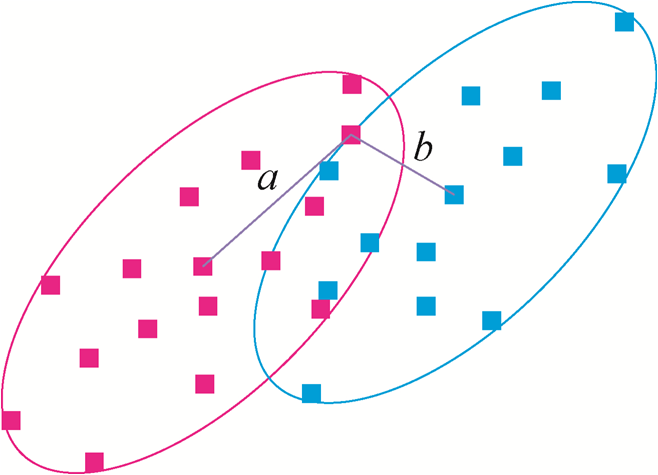
\includegraphics[width =0.6\hsize ]{maha.png}
\caption{2つの変数ベクトルの分散と距離}
\label{maha}
  \end{center}
\end{figure}

%具体的には,特徴量ベクトルを異方的に重み付けし,次のように$(l_x,l_y+1)$
%との相互相関に係数$C$を,$(l_x+1,l_y+1)$との相互相関に係数
%$D$をかける.
%
%\begin{eqnarray}
% {\bm K_{{\rm s}}'} = \left[
%\begin{array}{cccc}
% 1& & & \\
%  &C& & \\
%  & &1& \\
%  & & &D
%\end{array}
%                    \right]
% \left[
%  \begin{array}{c}
%   {\it K_{{\rm s}}}(0,0)\\
%   {\it K_{{\rm s}}}(0,1)\\
%   {\it K_{{\rm s}}}(1,0)\\
%   {\it K_{{\rm s}}}(1,1)
%  \end{array}
% \right]
%\end{eqnarray}
%
%これによって得られる特徴量ベクトル${\bm K'}$を
%新たな特徴量ベクトルとしてCSOMに入力する.
%\begin{eqnarray}
%{\bm K'} = \left[\begin{array}{ccc}
%      {\it K_{{\rm m}}} & {\bm K_{{\rm s}}'} & {\bm K_{{\rm f}}}
%           \end{array} \right]^{\mathrm{T}}
%\end{eqnarray}

\section{複素内積での勝者クラス決定法}
CSOMで各特徴量ベクトルの入力に対して勝者クラスを決定する方法には2通りある.
特徴量ベクトルと参照ベクトルのユークリッド距離をとり最小となるクラス
$\tilde{c}_E$を選択する方法(式(\ref{192027_15Feb15}))と,
特徴量ベクトルと参照ベクトルの複素内積を
とり最大となるクラス$\tilde{c}_I$を選択する方法\cite{2010Yoshida}である.
\begin{eqnarray}
\tilde{c}_I = \argmax_{c} \left( \left|
 \frac{{\bm K}^{\dagger}\cdot{\bm w_c}}{ \|{\bm K}\| \| {\bm w_c} \| }
                                   \right| \right)
\end{eqnarray}
従来の地雷可視化システムでは前者を選択していた.
しかし,本報告で提案するシステムではコヒーレンスにより敏感な後者の方が有
効である\cite{aoyagi}と予想される.図\ref{ip}において,コヒーレンスのあ
る実線ベクトル(a)とコヒーレンスのない破線ベクトル(b)を扱う際,ユークリッド距離
による勝者クラス決定法では実部があるために実軸投射したときに大きい(b)が勝
者となる.しかし,コヒーレンスを重視する,複素内積による勝者クラス決定法
では,複素ベクトルのノルムが大きい(a)が勝者となる.

\begin{figure}[btp]
 \begin{center}
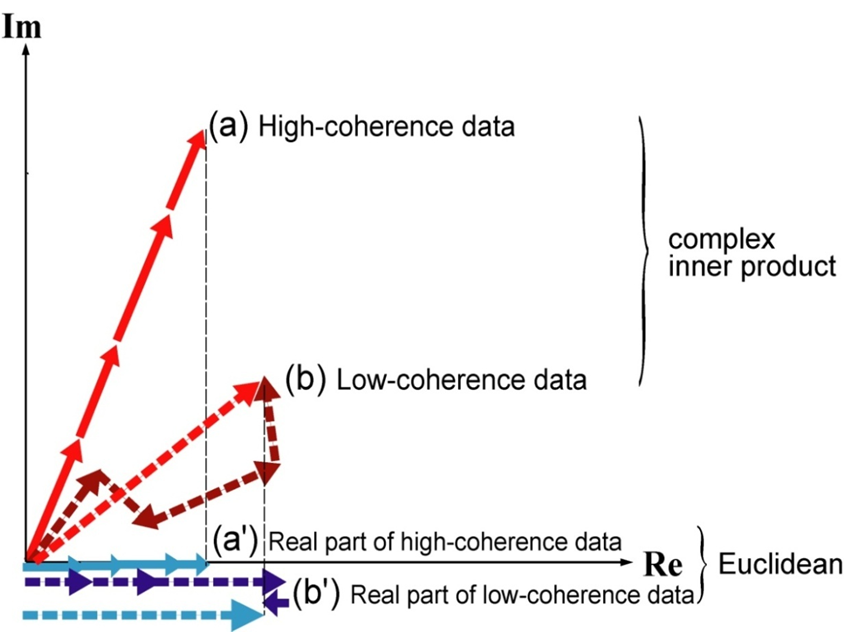
\includegraphics[width =0.6\hsize ]{innerproduct.png}
\caption{複素内積が有利に働く場合}
\label{ip}
  \end{center}
\end{figure}

次に,本手法で前項で説明した異方的重み付けを行う場合の条件式を以下に表す.
\begin{eqnarray}
\tilde{c}_I &=& \argmax_{c} \left( \left|
\frac{\left({\Sigma_w}^{-\frac{1}{2}}{\bm K}\right)^{\dagger}\cdot
\left({\Sigma_w}^{-\frac{1}{2}}{\bm w_c}\right)
}{ \|{\Sigma_w}^{-\frac{1}{2}}{\bm K}\| \|{\Sigma_w}^{-\frac{1}{2}}{\bm w_c} \| }
                                   \right| \right)\\
 &=& \argmax_{c} \left( \left|
\frac{{\bm K}^{\dagger}{\Sigma_w}^{-\frac{1}{2}
\dagger}{\Sigma_w}^{-\frac{1}{2}}\cdot{\bm w_c}
}{ \sqrt{{\bm K}^{\dagger}{\Sigma_w}^{-1}{\bm K}}\sqrt{{\bm
w_c}^{\dagger}{\Sigma_w}^{-1}{\bm w_c}} }
                                   \right| \right)\\
 &=& \argmax_{c} \left( \left|
\frac{{\bm K}^{\dagger}{\Sigma_w}^{-1}\cdot{\bm w_c}
}{ \sqrt{{\bm K}^{\dagger}{\Sigma_w}^{-1}{\bm K}}\sqrt{{\bm
w_c}^{\dagger}{\Sigma_w}^{-1}{\bm w_c}} }
                                   \right| \right)
\end{eqnarray}

本稿では,異方的重み付けを行う・行わない,勝者クラスの決定をユークリッド距
離で定める・複素内積で定めるの計4通りの手法を比較した.
\section{1次元アレイアンテナ式地雷可視化システムの高速化と保守性の向上}
節\ref{1array_before}で1次元アレイアンテナ式地雷可視化システムは試作され
たが,計測時間は462
点に15分を必要とし,反復実験を行うにはまだ高速化が不十分であると考えられ
た.
また,スイッチング部の制御回路に端子台が用いられており,回路箱の振動による信
号線の抜けが頻発していた.どのメカニカルスイッチが作動しているかを表示す
るLEDボードも直感的ではなかった.

これらの問題を解決するために,1次元アレイアンテナ式地雷可視化システムの
改良を行った.まず,図\ref{so2-2}に示すように,
高速化のネックとなっていたy軸方向へのアクチュエータ
動作をモジュール化した.以前はPCから直接プログラムでモータにON/OFF
の信号を送ることでパルスを生成し動作させていた.しかし,他のプログラムとの兼ね
合いで周期が10msecとなっており,一度に伸展させる7mm(700回転)のために1400周
期,14秒間待つ必要があった.そこで,指定された回転数分モータードライバを
運転する回路を組
み込み,PCからは動かしたい回転数をその回路に指示するだけで済むようにした.
これにより1.4秒で7mm伸展させることができるようになった.

\begin{figure}[btp]
 \begin{center}
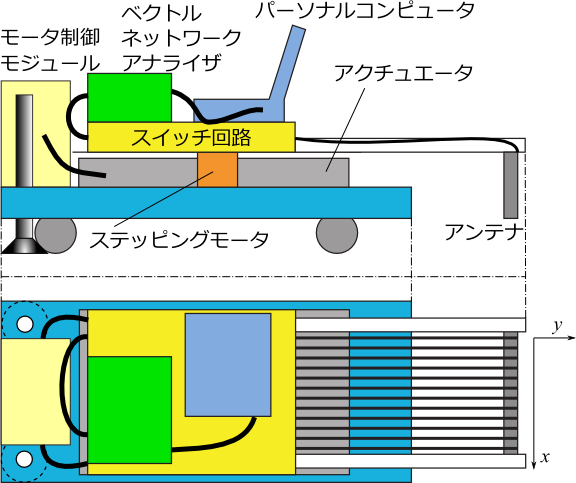
\includegraphics[width =0.6\hsize ]{so2-2.png}
\caption{モータ制御モジュールを追加した1次元アレイアンテナ式地雷可視化システム}
\label{so2-2}
  \end{center}
\end{figure}

次に,スイッチング回路箱を作り直し,挟み込み式であった信号線の端子台を廃し
ゆるみの少ないピン差し込み式に全て変更した.電源線は基板に直接ハンダ付けさ
れていたので,これもピン差し込み式に変更し,メンテナンス性を向上させた.

また,LED表示器を製作し,図\ref{LED}のような全てのスイッチが今何番に
切り替わっているかを表示していた以前のものから,図\ref{LED2}に表される,
スイッチの切り替えにより
経路が成立した時のみに光る直感的に分かりやすい仕様に変更した.

\begin{figure}[btp]
 \begin{center}
  \begin{tabular}{c}
   \begin{minipage}{0.5\hsize}
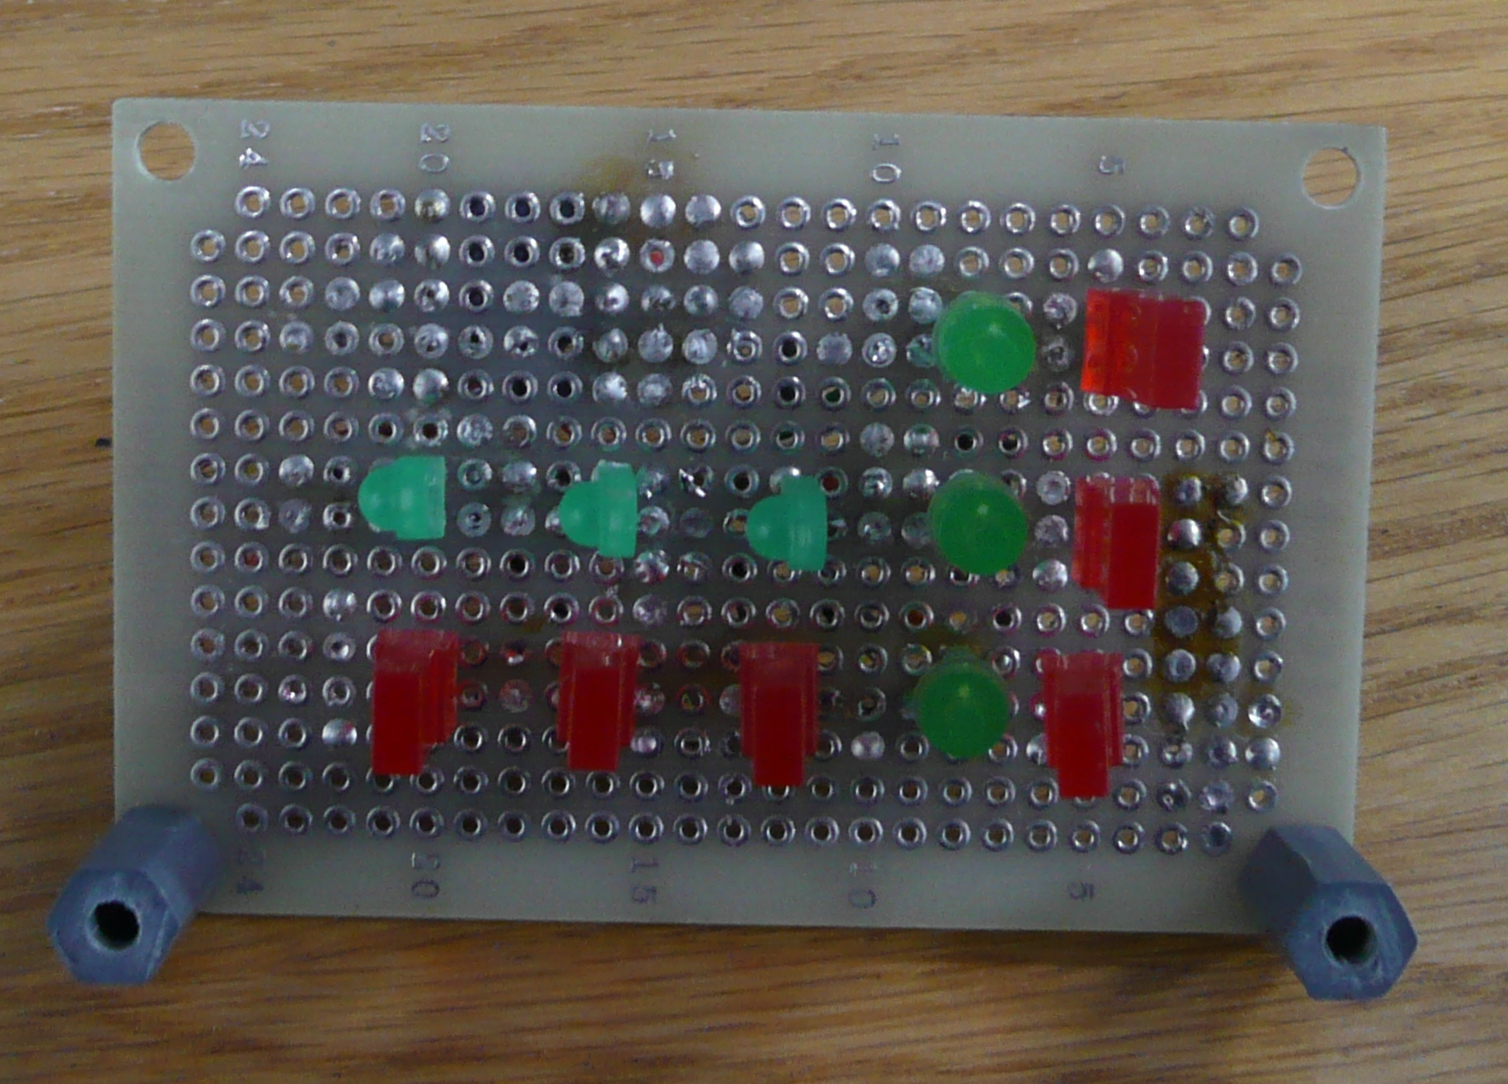
\includegraphics[width =\hsize ]{LED.png}
\caption{改良前のLEDボード}
\label{LED}      
   \end{minipage}
   \begin{minipage}{0.4\hsize}
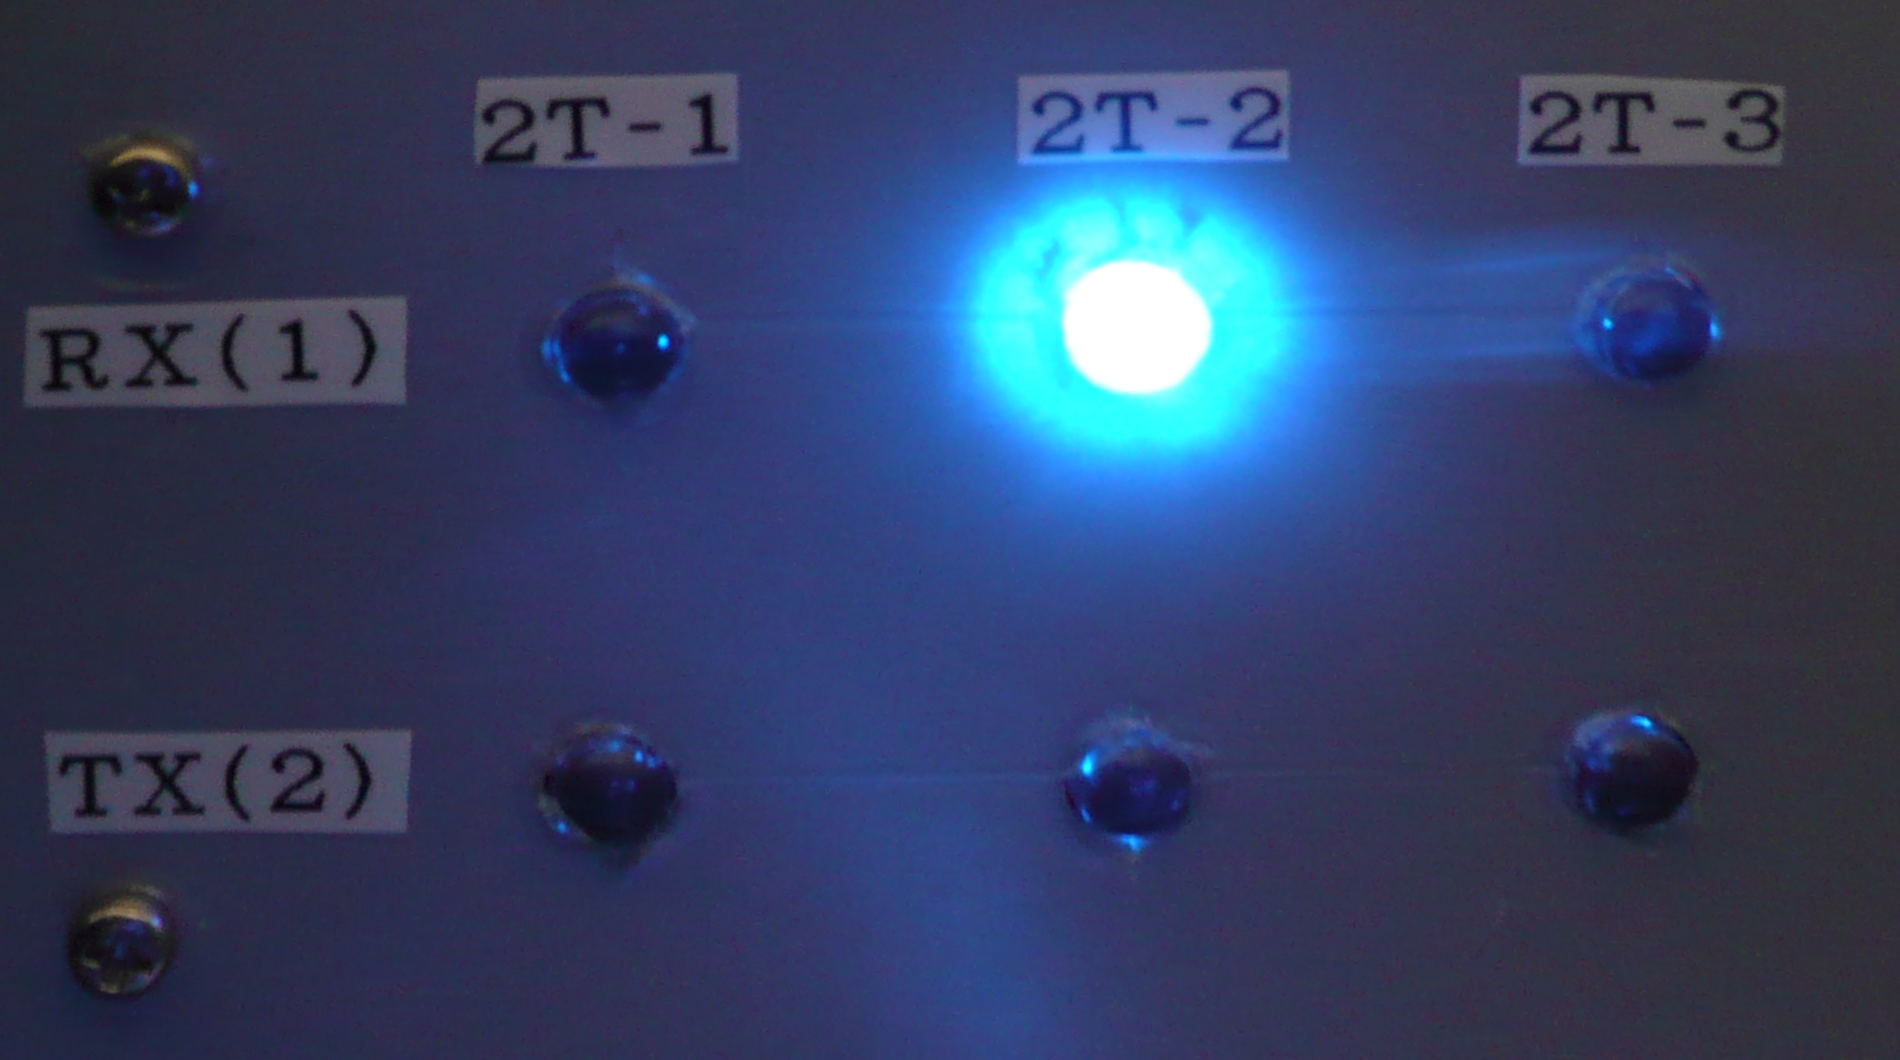
\includegraphics[width =\hsize ]{LED2.png}
\caption{改良後のLED表示器}
\label{LED2}          
   \end{minipage}
  \end{tabular}
 \end{center}
\end{figure}

\newpage
\chapter{模擬地雷計測実験}
\section{実験方法}
図\ref{landmine}のように,外径40cmの立方体型の植木鉢を用意し,そこに渇い
た土を入れ模擬地雷
を埋設した.土には小石や小枝などの他の散乱源も多数存在している.フロント
エンドの高さはこの地面にほぼ接するような距離になっている.埋設する模擬地雷は
直径8cmの上面円形の形状をし,素材はプラスチックである.
\begin{figure}[hbtp]
 \begin{center}
 \includegraphics[width =0.8\hsize ]{landmine.png}
\caption{実験に用いた環境と模擬地雷埋設}
\label{landmine}
 \end{center}
\end{figure}
\section{計測結果}
図\ref{mine-raw}〜図\ref{direct-raw}は,GPRからベクトルネットワークアナライザを通じて得られた振幅と
位相のデータを補正前の段階で画像として表示したものである.アンテナの
個体差が縦縞となって表れているのが確認できる.図\ref{mine-raw}は模擬地雷を埋設した
地面を計測したもの,図\ref{none-raw}は地雷を埋設せずに地面を計測したもの,図\ref{direct-raw}は
アンテナ下90cmに何も遮るものがない空間を計測したものである.

この何もない空間を計測したデータを直接結合の補正として用いてdata6を補正
した結果が図\ref{mine6-hosei}である.前処理では縦縞を軽減することはでき
るものの,完全に除去することはできないことが分かる.
\begin{figure}[hbtp]
 \begin{center}
     \begin{minipage}[c]{0.19\hsize}
      data1,振幅
  \end{minipage}
     \begin{minipage}[c]{0.79\hsize}
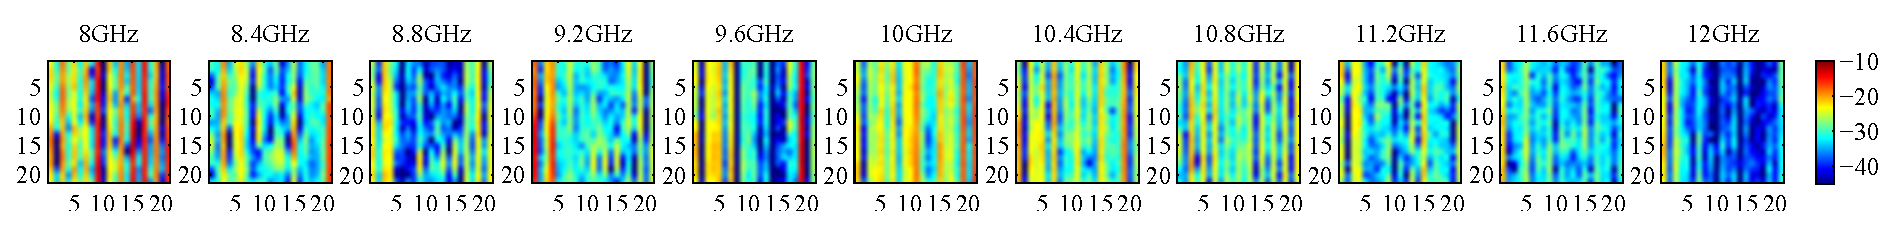
\includegraphics[width = \hsize ]{20150204_mine1_raw_a.eps}
  \end{minipage}
\\
     \begin{minipage}[c]{0.19\hsize}
data1,位相
  \end{minipage}
     \begin{minipage}[c]{0.8\hsize}
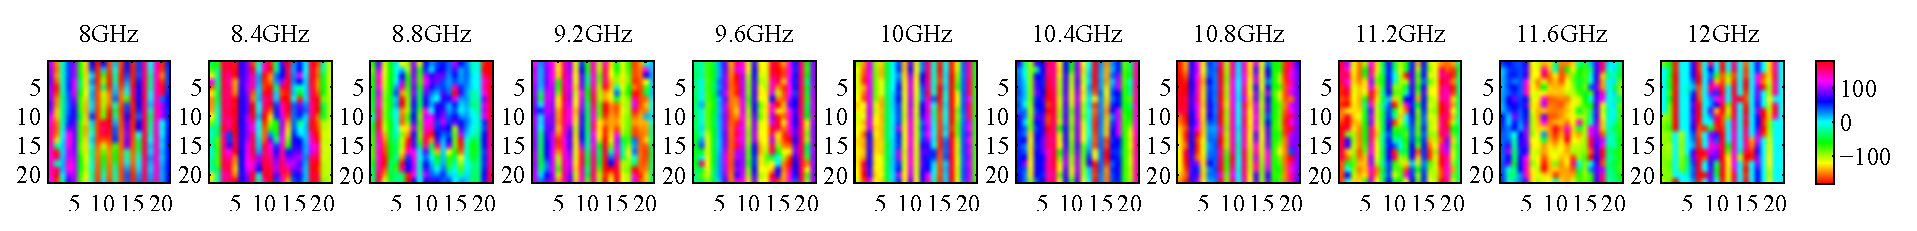
\includegraphics[width =\hsize ]{20150204_mine1_raw_p.eps}
  \end{minipage}
\end{center}
\end{figure}
\begin{figure}[bhtp]
 \begin{center}
     \begin{minipage}[c]{0.19\hsize}
      data2,振幅
  \end{minipage}
     \begin{minipage}[c]{0.79\hsize}
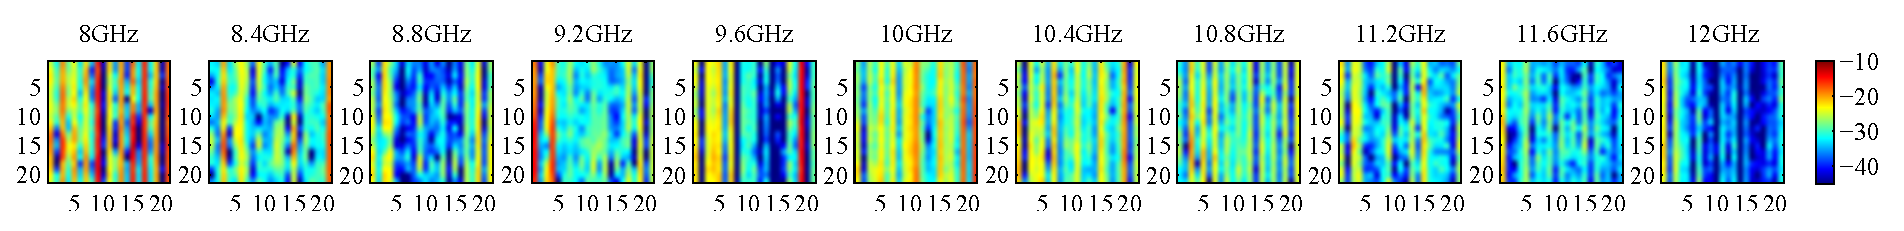
\includegraphics[width = \hsize ]{20150204_mine2_raw_a.eps}
  \end{minipage}
\\
     \begin{minipage}[c]{0.19\hsize}
data2,位相
  \end{minipage}
     \begin{minipage}[c]{0.8\hsize}
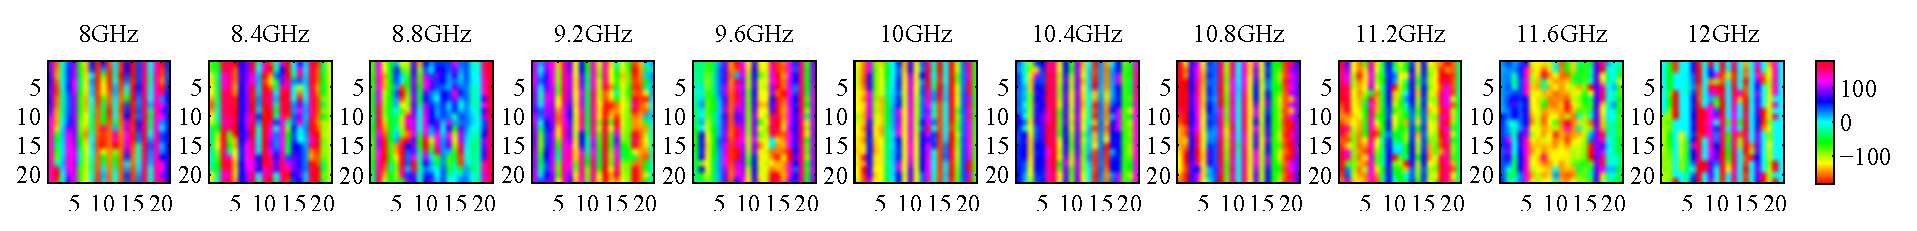
\includegraphics[width =\hsize ]{20150204_mine2_raw_p.eps}
  \end{minipage}
\end{center}
\end{figure}
\begin{figure}[bhtp]
 \begin{center}
     \begin{minipage}[c]{0.19\hsize}
      data3,振幅
  \end{minipage}
     \begin{minipage}[c]{0.79\hsize}
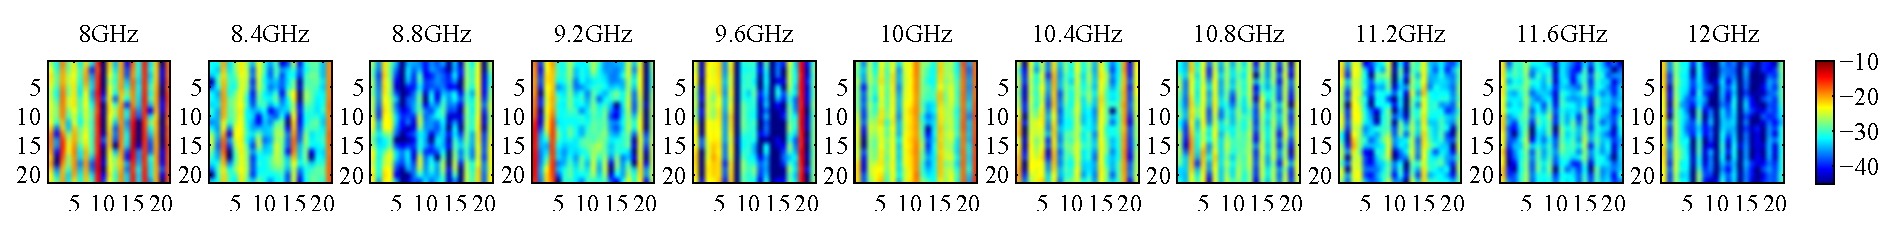
\includegraphics[width = \hsize ]{20150204_mine3_raw_a.eps}
  \end{minipage}
\\
     \begin{minipage}[c]{0.19\hsize}
data3,位相
  \end{minipage}
     \begin{minipage}[c]{0.8\hsize}
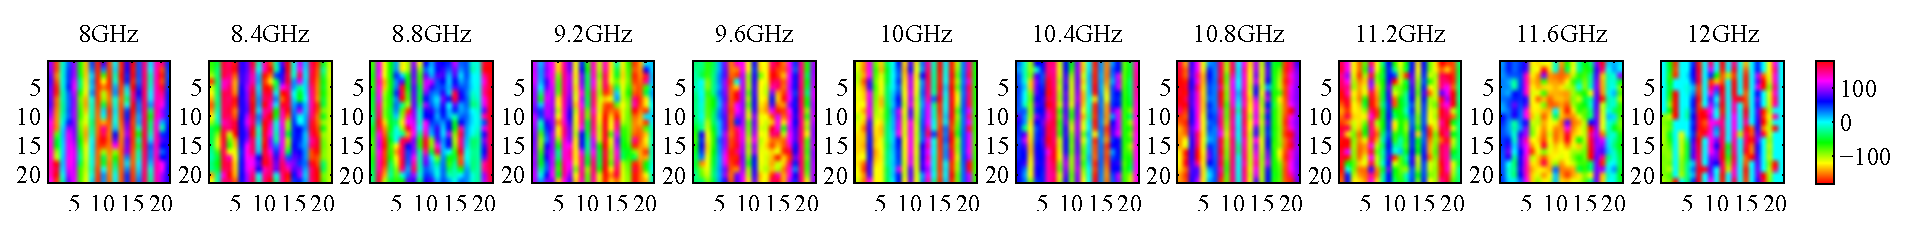
\includegraphics[width =\hsize ]{20150204_mine3_raw_p.eps}
  \end{minipage}
\end{center}
\end{figure}
\begin{figure}[bhtp]
 \begin{center}
     \begin{minipage}[c]{0.19\hsize}
      data4,振幅
  \end{minipage}
     \begin{minipage}[c]{0.79\hsize}
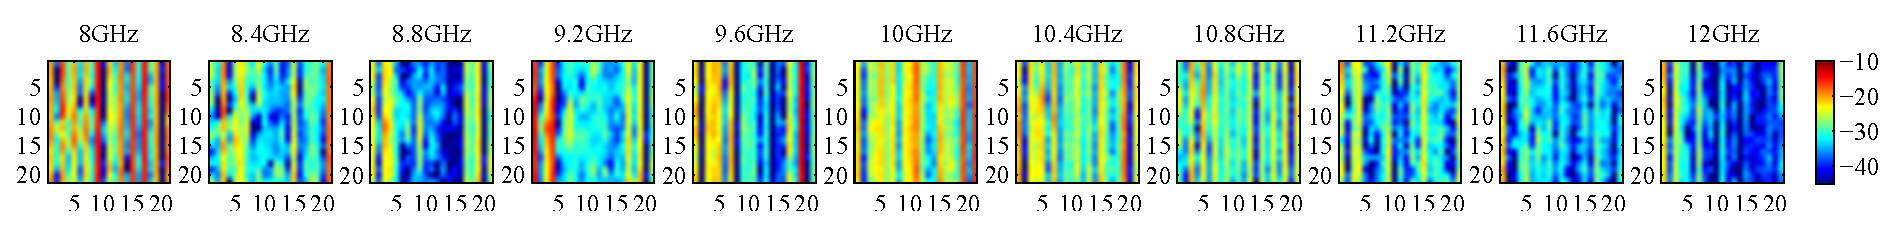
\includegraphics[width = \hsize ]{20150204_mine4_raw_a.eps}
  \end{minipage}
\\
     \begin{minipage}[c]{0.19\hsize}
data4,位相
  \end{minipage}
     \begin{minipage}[c]{0.8\hsize}
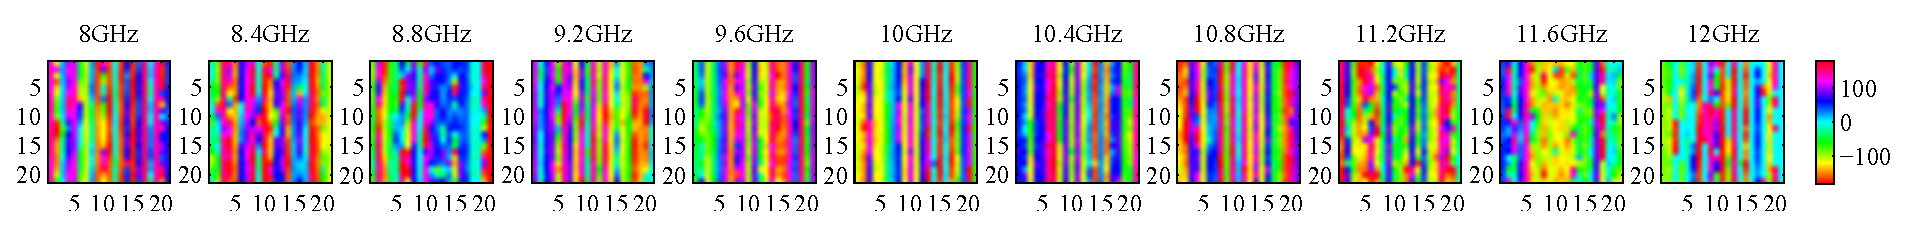
\includegraphics[width =\hsize ]{20150204_mine4_raw_p.eps}
  \end{minipage}
\end{center}
\end{figure}
\begin{figure}[bhtp]
 \begin{center}
     \begin{minipage}[c]{0.19\hsize}
      data5,振幅
  \end{minipage}
     \begin{minipage}[c]{0.79\hsize}
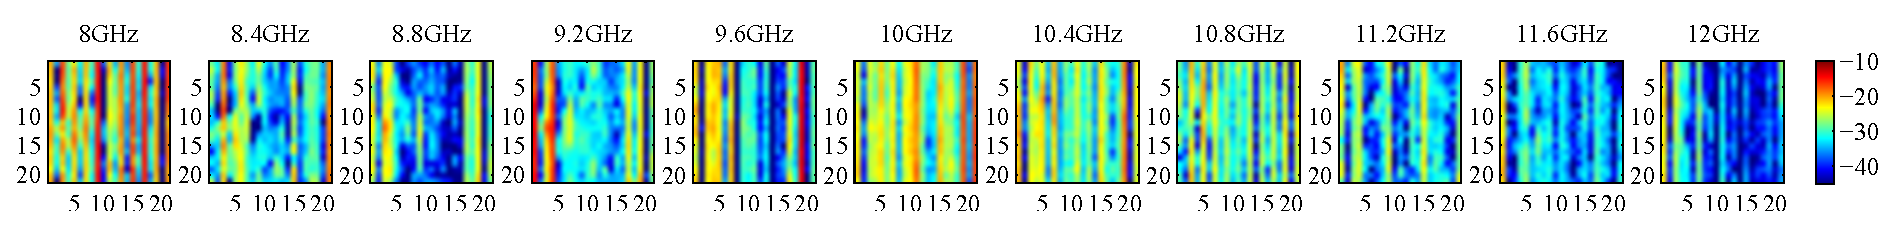
\includegraphics[width = \hsize ]{20150204_mine5_raw_a.eps}
  \end{minipage}
\\
     \begin{minipage}[c]{0.19\hsize}
data5,位相
  \end{minipage}
     \begin{minipage}[c]{0.8\hsize}
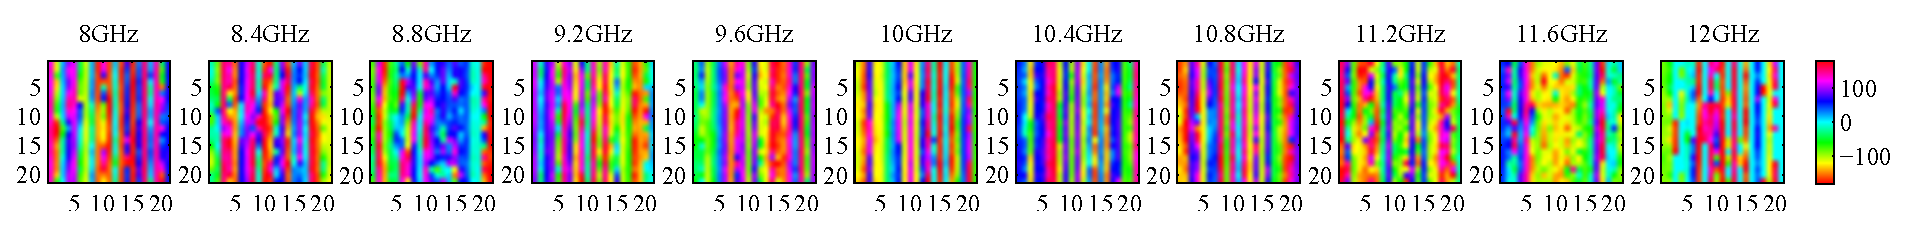
\includegraphics[width =\hsize ]{20150204_mine5_raw_p.eps}
  \end{minipage}
\end{center}
\end{figure}
\begin{figure}[hbtp]
 \begin{center}
     \begin{minipage}[c]{0.19\hsize}
      data6,振幅
  \end{minipage}
     \begin{minipage}[c]{0.79\hsize}
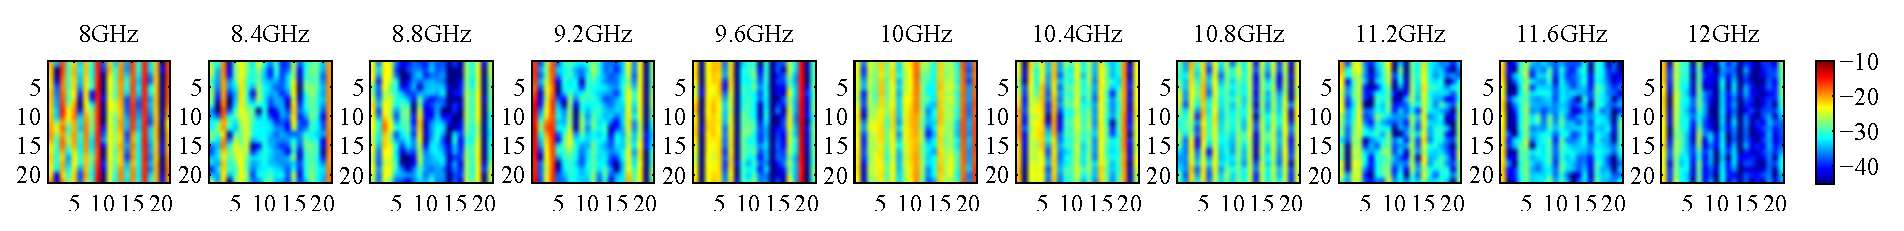
\includegraphics[width = \hsize ]{20150204_mine6_raw_a.eps}
  \end{minipage}
\\
     \begin{minipage}[c]{0.19\hsize}
data6,位相
  \end{minipage}
     \begin{minipage}[c]{0.8\hsize}
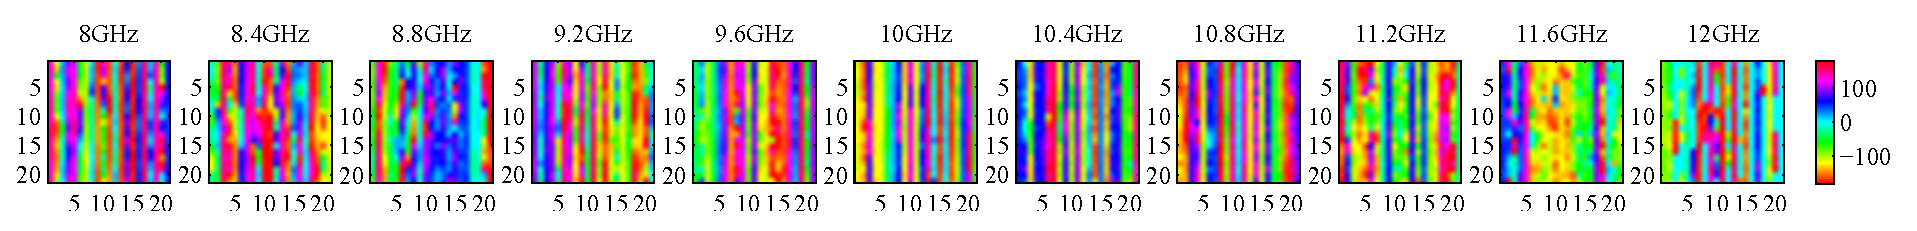
\includegraphics[width =\hsize ]{20150204_mine6_raw_p.eps}
  \end{minipage}
\end{center}
\end{figure}
\begin{figure}[hbtp]
 \begin{center}
     \begin{minipage}[c]{0.19\hsize}
      data7,振幅
  \end{minipage}
     \begin{minipage}[c]{0.79\hsize}
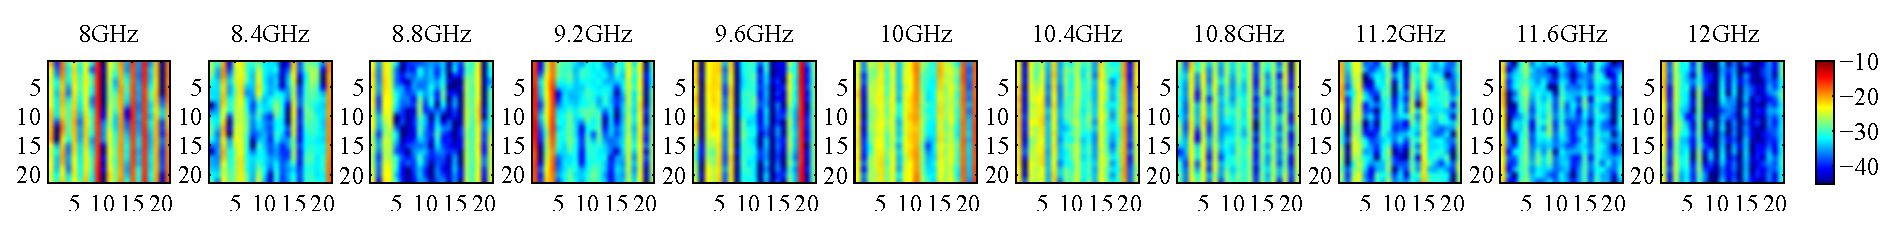
\includegraphics[width = \hsize ]{20150204_mine7_raw_a.eps}
  \end{minipage}
\\
     \begin{minipage}[c]{0.19\hsize}
data7,位相
  \end{minipage}
     \begin{minipage}[c]{0.8\hsize}
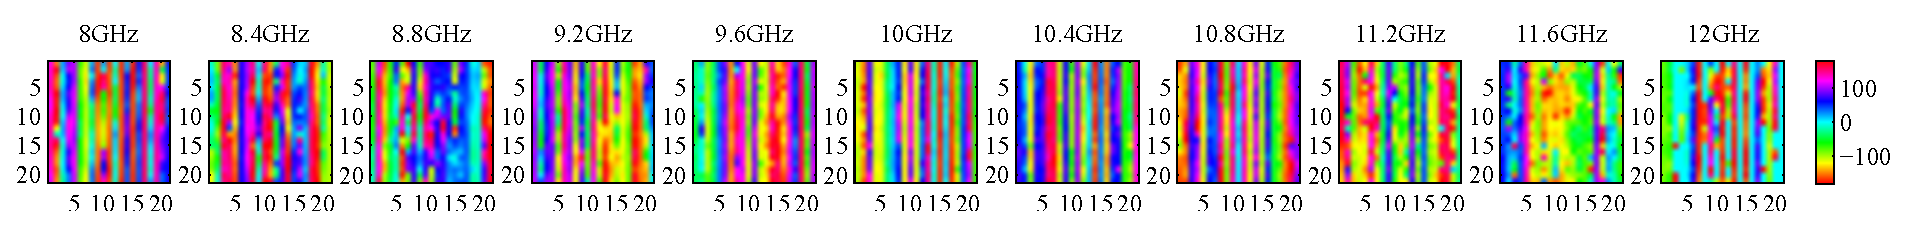
\includegraphics[width =\hsize ]{20150204_mine7_raw_p.eps}
  \end{minipage}
\end{center}
\end{figure}
\begin{figure}[hbtp]
 \begin{center}
     \begin{minipage}[c]{0.19\hsize}
      data8,振幅
  \end{minipage}
     \begin{minipage}[c]{0.79\hsize}
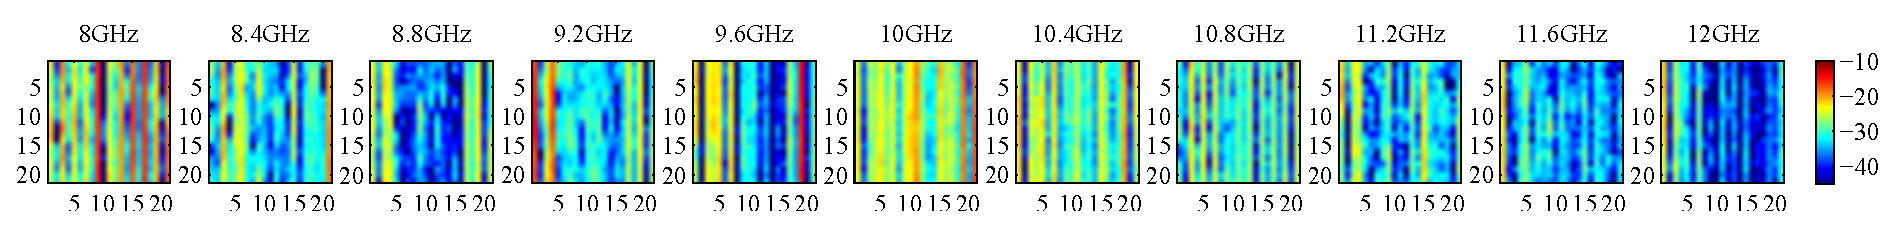
\includegraphics[width = \hsize ]{20150204_mine8_raw_a.eps}
  \end{minipage}
\\
     \begin{minipage}[c]{0.19\hsize}
data8,位相
  \end{minipage}
     \begin{minipage}[c]{0.8\hsize}
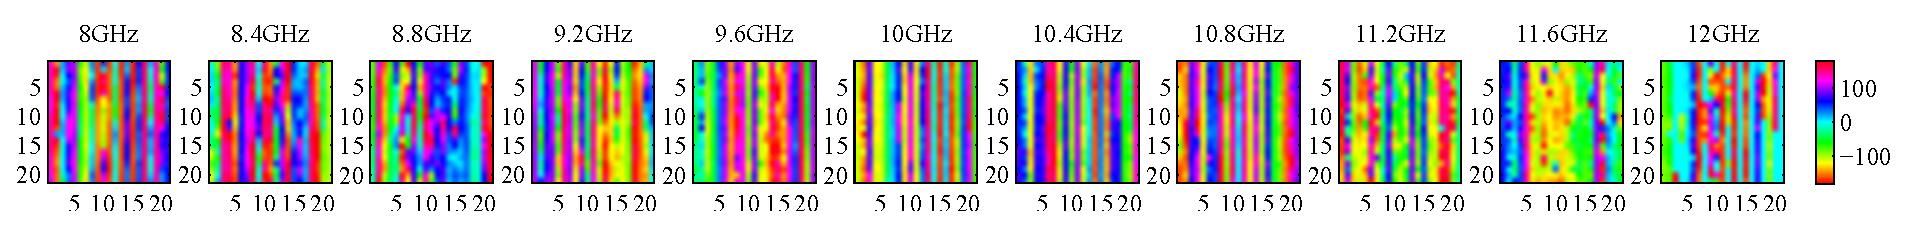
\includegraphics[width =\hsize ]{20150204_mine8_raw_p.eps}
  \end{minipage}
\end{center}
\end{figure}
\begin{figure}[hbtp]
 \begin{center}
     \begin{minipage}[c]{0.19\hsize}
      data9,振幅
  \end{minipage}
     \begin{minipage}[c]{0.79\hsize}
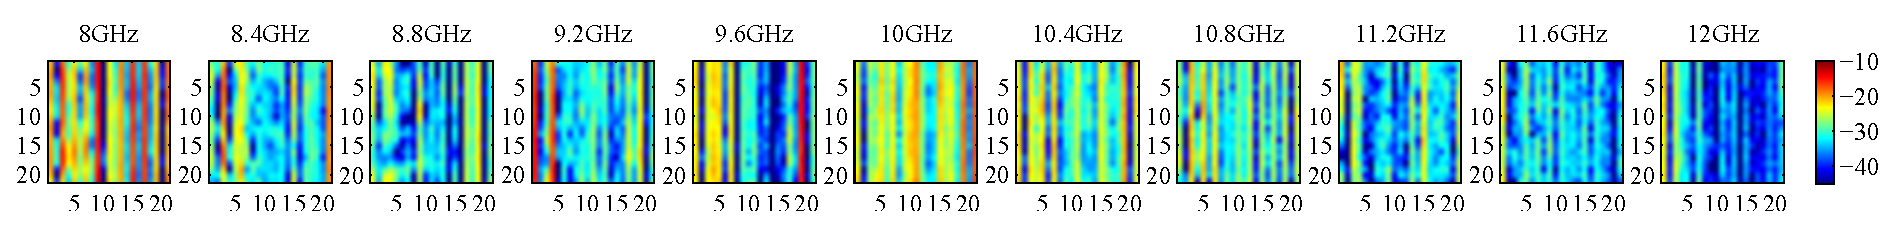
\includegraphics[width = \hsize ]{20150204_mine9_raw_a.eps}
  \end{minipage}
\\
     \begin{minipage}[c]{0.19\hsize}
data9,位相
  \end{minipage}
     \begin{minipage}[c]{0.8\hsize}
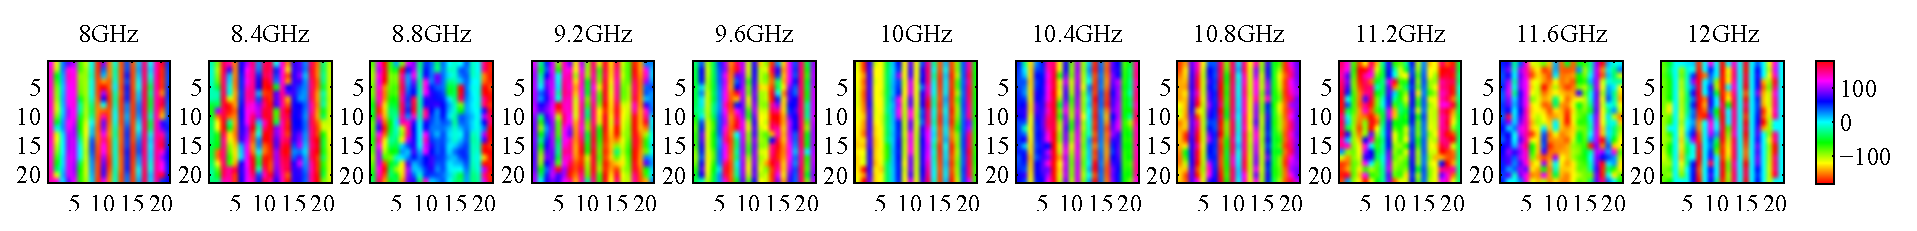
\includegraphics[width =\hsize ]{20150204_mine9_raw_p.eps}
  \end{minipage}
\end{center}
\end{figure}
\begin{figure}[hbtp]
 \begin{center}
     \begin{minipage}[c]{0.19\hsize}
      data10,振幅
  \end{minipage}
     \begin{minipage}[c]{0.79\hsize}
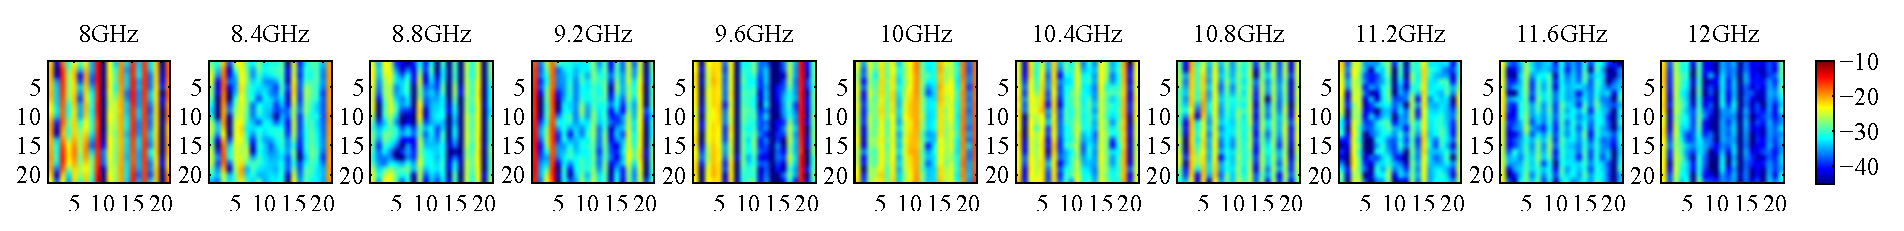
\includegraphics[width = \hsize ]{20150204_mine10_raw_a.eps}
  \end{minipage}
\\
     \begin{minipage}[c]{0.19\hsize}
data10,位相
  \end{minipage}
     \begin{minipage}[c]{0.8\hsize}
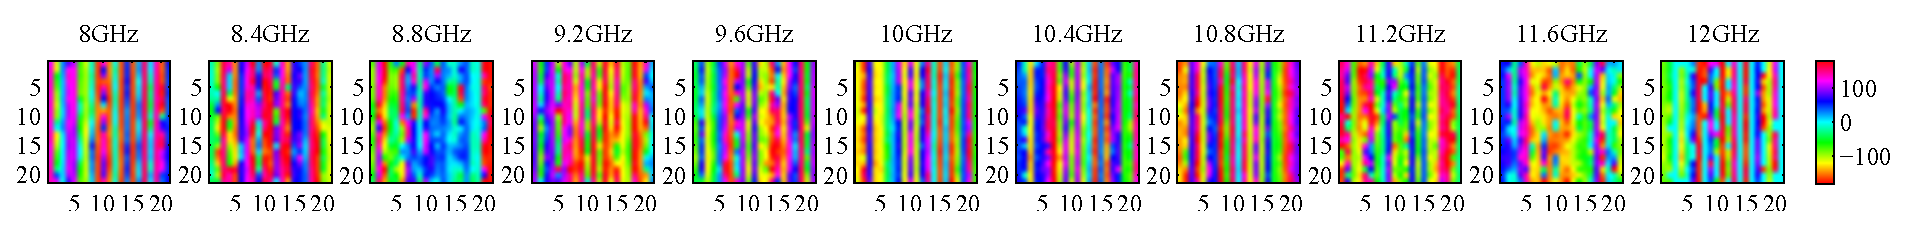
\includegraphics[width =\hsize ]{20150204_mine10_raw_p.eps}
  \end{minipage}
\\
\caption{模擬地雷を埋設して計測したデータ}
\label{mine-raw}
 \end{center}
\end{figure}
\begin{figure}[hbtp]
 \begin{center}
     \begin{minipage}[c]{0.19\hsize}
振幅
  \end{minipage}
     \begin{minipage}[c]{0.79\hsize}
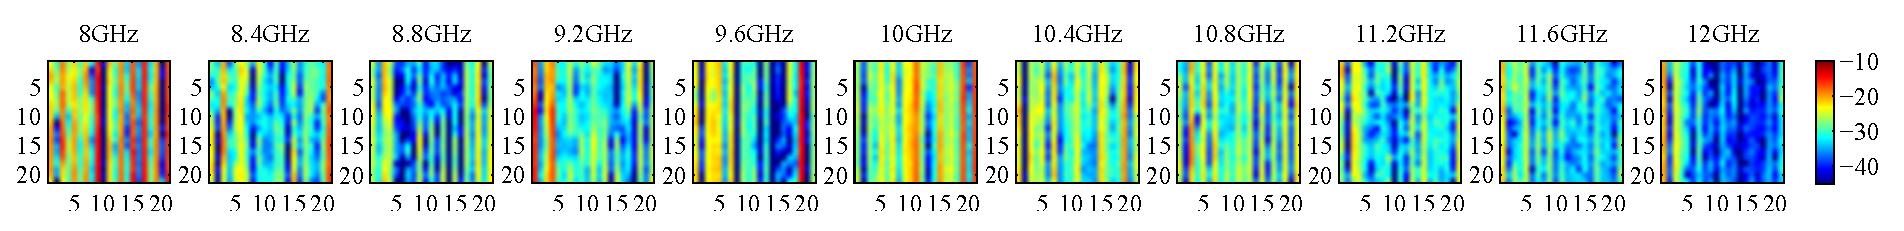
\includegraphics[width = \hsize ]{20150204_none1_raw_a.eps}
  \end{minipage}
\\
     \begin{minipage}[c]{0.19\hsize}
位相
  \end{minipage}
     \begin{minipage}[c]{0.8\hsize}
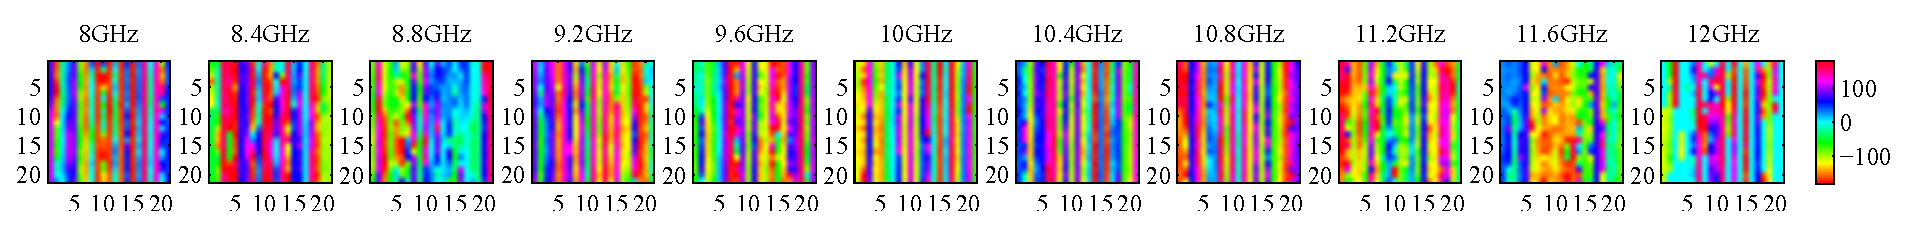
\includegraphics[width =\hsize ]{20150204_none1_raw_p.eps}
  \end{minipage}
\caption{模擬地雷のない地面を計測したデータ}
\label{none-raw} 
 \end{center}
\end{figure}
\begin{figure}[hbtp]
 \begin{center}
     \begin{minipage}[c]{0.19\hsize}
振幅
  \end{minipage}
     \begin{minipage}[c]{0.79\hsize}
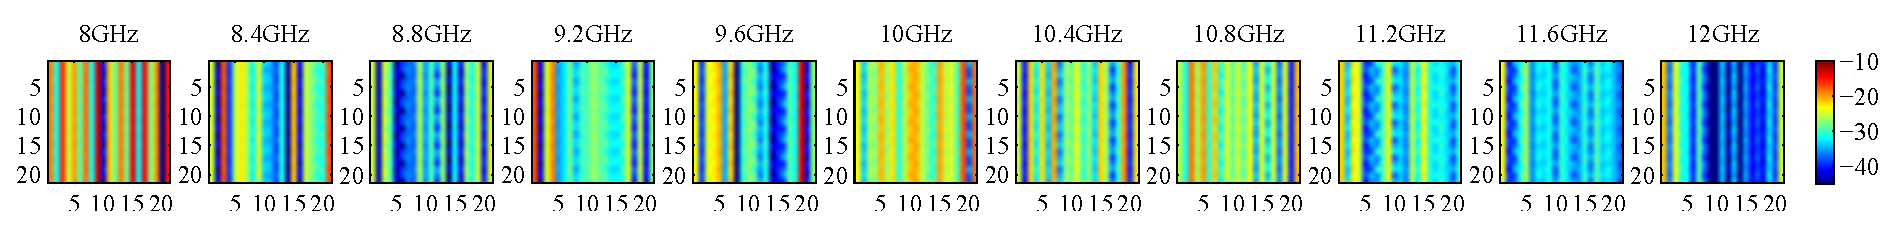
\includegraphics[width = \hsize ]{20150206_direct2_raw_a.eps}
  \end{minipage}
\\
     \begin{minipage}[c]{0.19\hsize}
位相
  \end{minipage}
     \begin{minipage}[c]{0.8\hsize}
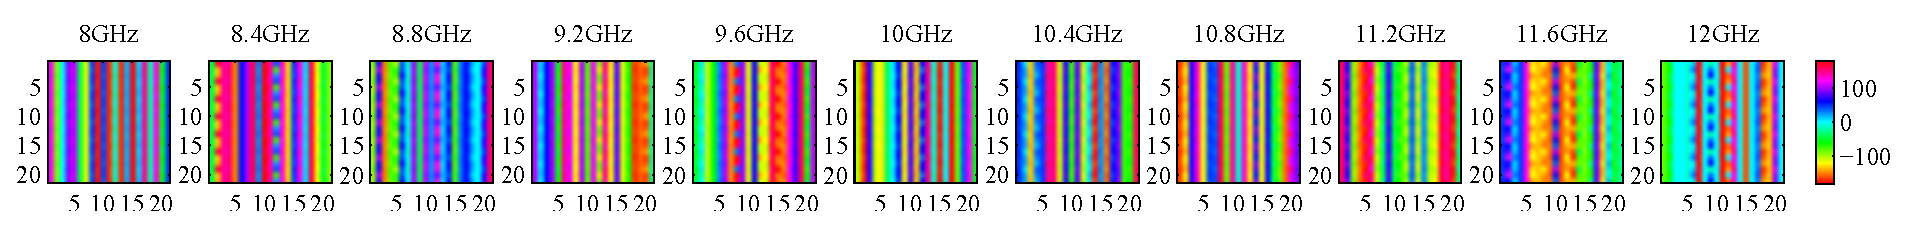
\includegraphics[width =\hsize ]{20150206_direct2_raw_p.eps}
  \end{minipage}
\caption{空中を計測したデータ}
\label{direct-raw}
 \end{center}
\end{figure}
\begin{figure}[hbtp]
 \begin{center}
     \begin{minipage}[c]{0.19\hsize}
振幅
  \end{minipage}
     \begin{minipage}[c]{0.79\hsize}
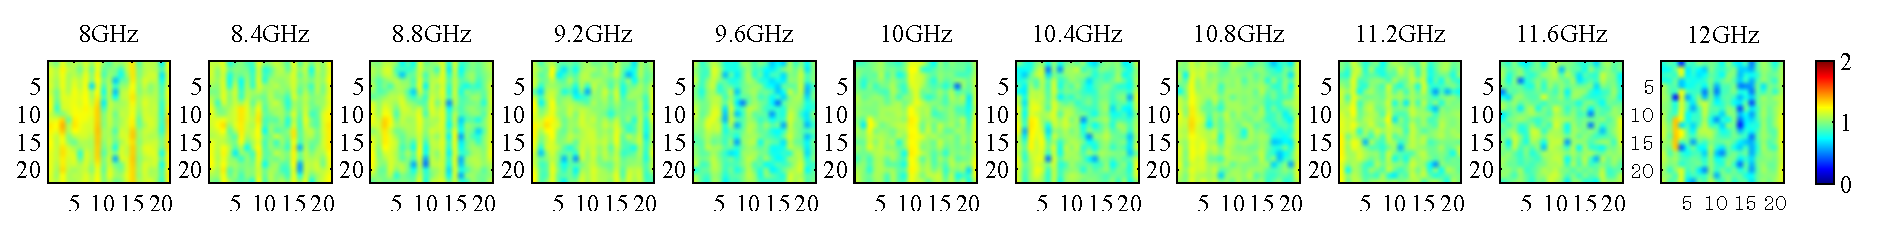
\includegraphics[width = \hsize ]{20150204_mine6_Bhosei_a.eps}
  \end{minipage}
\\
     \begin{minipage}[c]{0.19\hsize}
位相
  \end{minipage}
     \begin{minipage}[c]{0.8\hsize}
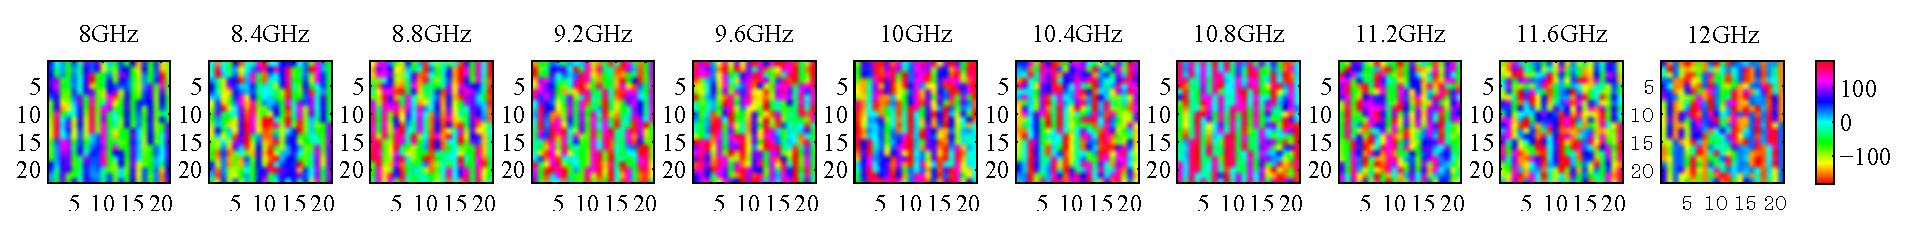
\includegraphics[width =\hsize ]{20150204_mine6_Bhosei_p.eps}
  \end{minipage}
\caption{data6を補正した後の画像}
\label{mine6-hosei}
 \end{center}
\end{figure}

\section{自己組織化マップの使用に対する2つの新手法と区分画像}
前処理を適用した後のdata6に対し,特徴量ベクトルの
異方的重み付けと複素内積での勝者クラス決定法を試した.
まず,ユークリッド距離で勝者クラスを決定する従来の手法で異方的重み付け
を行ったSOMの結果が図\ref{aniso-e}である.\\
\begin{figure}[btp]
 \begin{center}
\begin{tabular}{cc}
   \begin{minipage}{0.5\hsize}
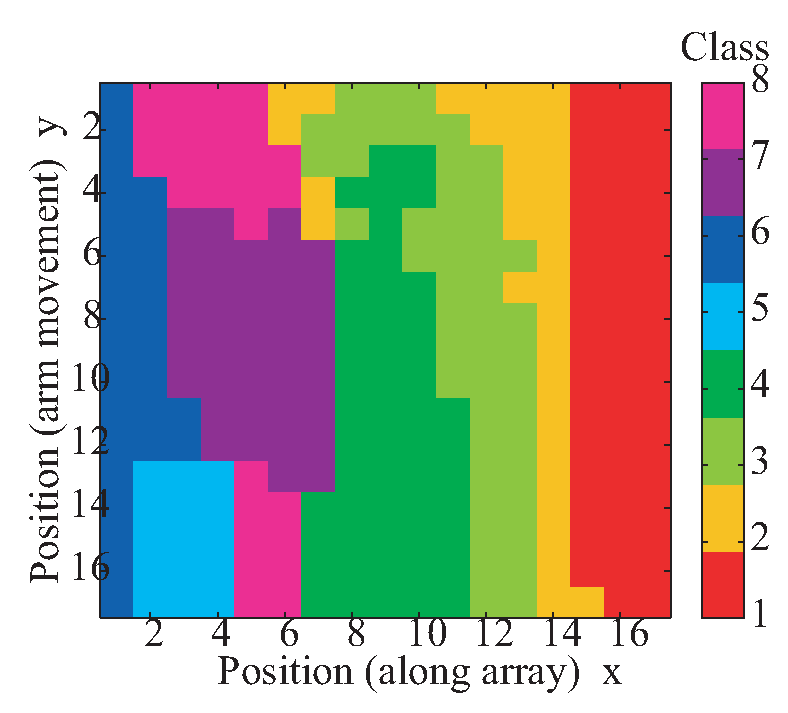
\includegraphics[width =\hsize ]{SOM_mine6_02005_e_raw.eps}
\centering\textmd{異方的重み付けなし}
   \end{minipage}
&
   \begin{minipage}{0.5\hsize}
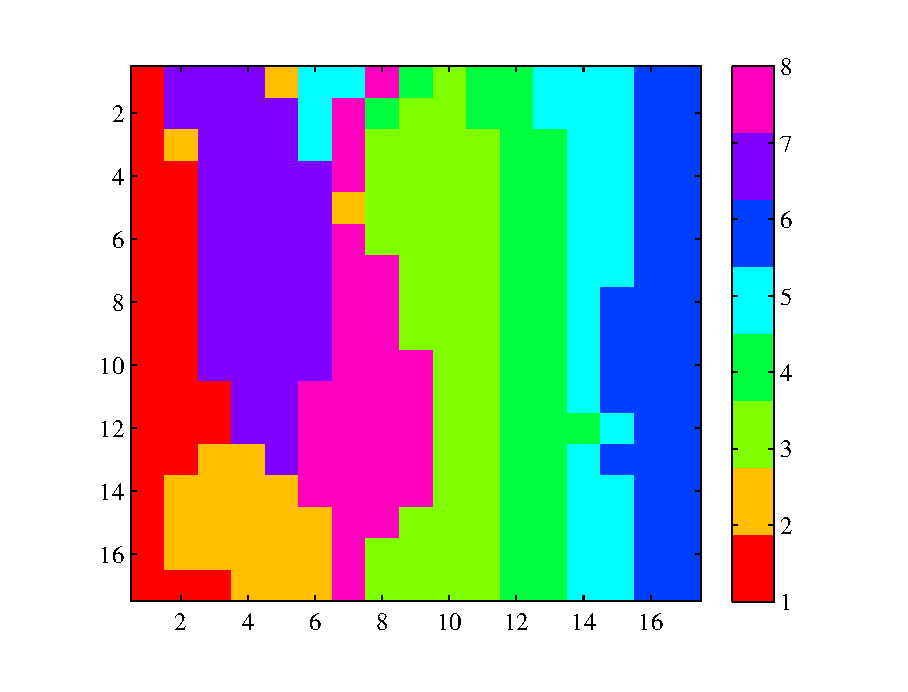
\includegraphics[width =\hsize ]{SOM_mine6_02005_e_wsqrt.eps}
\centering\textmd{異方的重み付けあり}
   \end{minipage}
\end{tabular}
\caption{ユークリッド距離で勝者クラスを決定した時の異方的重み付け結果}
\label{aniso-e}
 \end{center}
\end{figure}

次に,複素内積で勝者クラスを決定する手法により異方的重み付けを行った結果
が図\ref{aniso-i}である.

\begin{figure}[btp]
 \begin{center}
\begin{tabular}{cc}
   \begin{minipage}{0.5\hsize}
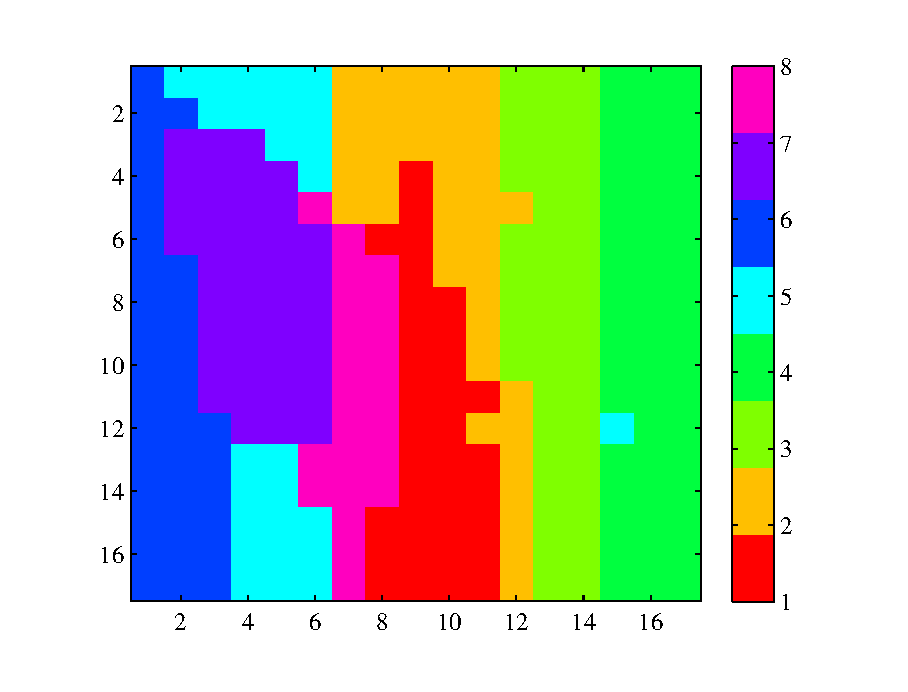
\includegraphics[width =\hsize ]{SOM_mine6_02005_i_raw.eps}
\centering\textmd{異方的重み付けなし}
   \end{minipage}
&
   \begin{minipage}{0.5\hsize}
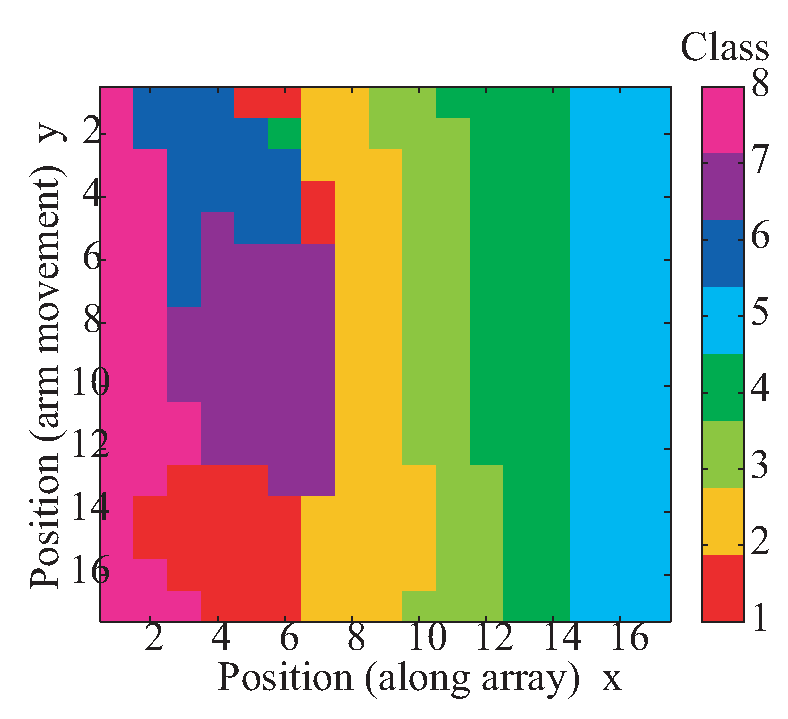
\includegraphics[width =\hsize ]{SOM_mine6_02005_i_wsqrt.eps}
\centering\textmd{異方的重み付けあり}
   \end{minipage}
\end{tabular}
\caption{複素内積で勝者クラスを決定した時の異方的重み付け結果}
\label{aniso-i}
 \end{center}
\end{figure}
\newpage
\chapter{考察と今後の課題}
\section{考察}
\subsection{新型システムの有用性}
新型システムを改良する前は22列の計測に15分かかっていたが,改良の結果約5分
半で計測を終えることができた.まだ金属探知器を用いて人間が金属地雷を探知
するような速度で計測することはできていないが,金属探知器では詳細な形状は
分からない.この改良は有意義であったと考える.
\subsection{勝者クラスの決定法の選択によるCSOMの変化}
異方的重み付けを行うことにより,図\ref{aniso-e}において特に下半分につい
て顕著に縦縞の影響が軽減されていることを確認した.しかし,ユークリッド距
離においては異方的重み付けを行うことで地雷クラスの形状が歪んでしまっていた.

複素内積による勝者クラス決定法は,異方的重み付けを行わない場合には,
ユークリッド距離による勝者クラス決定法よりも形状が歪んでおり適さないようだが,異方
的重み付けを行った際には,最も地雷の形状を適切に判断できている.
以上より,4手法の比較において,異方的重み付けを行いつつ複素内積による勝
者クラス決定法を用いるのが安定して地雷を判別
できる手段であると確認できる.従って,異方的重み付けと複素内積による勝者
クラス決定法は併用するのが最適であると結論づける.
\section{今後の課題}
継続して計測速度を改善しつつ,アンテナ部の機構を見直し性能を向上させる.
また,データ数を増やして教師画像とし,
実際に未知画像を取得して地雷の判別率を算出し,実用性を検討する.
\section*{謝辞}
この研究を進めるにあたり,熱心にご指導をいただいた廣瀬明教授に感謝いたし
ます.システムの改良に際し回路面と数学面でご助力くださった西村さん,アクチュエー
タ制御回路とボックスを製作してくださった村田君,また,アドバイスや励
ましの言葉をくださった研究室の皆様にお礼申し上げます.

%\bibliography{myrefs}
\begin{thebibliography}{99}% 文献数が10未満の時 {9}
\bibitem{Arai} T. Susuki and I. Arai, "Advance on underground radars," IEICE
Transactions, vol.E74, no.2, pp.289-294, 1991.
\bibitem{2007TCounts} T. Counts, A. C. Gurbuz, W. R. Scott Jr.,
        J. H. McClellan and K. Kim, "Multistatic
ground-penetrating radar experiments," IEEE Transrations on Geoscience and
Remote Sensing, vol. 45, no. 10, pp. 2544-2553, October 2007.
\bibitem{chichi} C-C Chen, S. Nag, W. D. Burnside, J. I. Halman,
K. A. Shubert and L. Peters, Jr., "A Standoff, Focused-Beam Land Mine Radar,"
IEEE Transactions on Geoscience and Remote Sensing, vol.38, no.1, pp. 507-514, 2000.
\bibitem{JeroenYarovoy} Jeroen Groenenboom, Alexander Yarovoy,
"Data Processing and Imaging in GPR System Dedicated for Landmine
Detection," Subsurface Sensing Technologies and Applications, vol.3,
        no.4, pp. 387-402, 2002.
\bibitem{YaroboyLighthart} Alexander G. Yarovoy and  Leo P. Ligthart,
"Polarimetric video impulse radar for landmine detection,"
Subsurface Sensing Technologies and Applications, vol.3, no.4, pp. 271-293, 2002.
\bibitem{2004MSato} M. Sato, Y. Hamada, X. Feng, F. N. Kong, Z. Zeng and
        G. Fang, "GPR using an array an-
tenna for land-mine detection," Near Subsurface Geophysics, vol. 2,
        pp. 7-13, 2004.
 \bibitem{2005Sato} M. Sato, K. Takahashi, X. Feng and
        T. Kobayashi, "Dual sensor alis evaluation test in
        Afghanistan," IEEE Geoscience and Remote Sensing Society
        Newsletter, pp. 22-24, September 2005.
 \bibitem{2009Sato} M. Sato, K. Takahashi, "Development of
        Dual Sensors and Deployment in Mine Affected
        Countries," in {\it Anti-personal Landmine Detection for
        Humanitarian Demining}, pp. 27-44, 2009.
\bibitem{2007SMas} S. Masuyama and A. Hirose, "Walled LTSA array for rapid, high spatial resolution,
and phase sensitive imaging to visualize plastic landmines," IEEE Transactions
on Geoscience and Remote Sensing, vol. 45, no. 8, pp. 2536-2543, August 2007.
\bibitem{2008SMas} S. Masuyama, K. Yasuda and A. Hirose, "Multiple mode selection of
walled-ltsa array elements for high resolution imaging to visualize antipersonnel
plastic landmines," IEEE Geoscience and Remote Sensing Letters, vol. 5,
        no. 4, pp. 745-749, October 2008.
\bibitem{2009Nakano} Y. Nakano and A. Hirose, "Improvement of plastic
        landmine visualization performance by use of ring-csom and
        frequency-domain local correlation," IEICE Transactions on
        Electronics, vol. E92-C, no. 1, pp. 102-108, January 2009.
\bibitem{2010Nakano} Y. Nakano and A. Hirose, "Adaptive identification of
        landmine class by evaluating the total degree of conformity of
        ring-SOM," Australian Journal of Intelligent Information
        Processing Systems, pp. 23-28, December 2010.
\bibitem{ejiri} A. Ejiri and A. Hirose, "Landmine visualization
        system based on multiple complex-valued SOMs to integrate
        multimodal information," ICJNN The 2012 International Joint
        Conference on, pp. 1-7, June 2012.
\bibitem{2011Nakano} Y. Nakano and A. Hirose, "Taper-walled linearly
        tapered slot antenna," IEEE Journal of Selected Topics in
        Applied Earth Observations and Remote Sensing, pp. 779-784, 
        April 2011.
\bibitem{2010Yoshida} A. Hirose and S. Yoshida, "Generalization
        Characteristics of Complex-Valued Feedforward Neural Networks in
        Relation to Signal Coherence," IEEE Neural Networks and Learning
        Systems, vol.23, no.4, 541-551, April 2012.
\bibitem{aoyagi} T. Aoyagi, D. Radenamad, Y. Nakano and A. Hirose,
        "Complex-valued self-organizing map clustering using complex
        inner product in active mmillimeter-wave imaging," Int'l Joint
        Conference on Neural Networks (IJCNN) pp. 1346-1351 July 2010.
\end{thebibliography}
\renewcommand{\bibname}{発表文献}
\begin{thebibliography}{9}
\bibitem{koyama} E. Koyama, K. Matsuyama, A. Ejiri, and
        A. Hirose, "Landmine visualization system using complex-valued
        self-organizing map with one-dimensional array antenna," IEICE
        Neurocomputing, Technical Report, vol.113, no.500, 
        pp. 69-74, March 2014.
\end{thebibliography}
\end{document}
